%%%%%%%%%%%%%%%%%%%%%%%%%%%%%%%%%%%%%%%%%
% Masters/Doctoral Thesis 
% LaTeX Template
% Version 2.5 (27/8/17)
%
% This template was downloaded from:
% http://www.LaTeXTemplates.com
%
% Version 2.x major modifications by:
% Vel (vel@latextemplates.com)
%
% This template is based on a template by:
% Steve Gunn (http://users.ecs.soton.ac.uk/srg/softwaretools/document/templates/)
% Sunil Patel (http://www.sunilpatel.co.uk/thesis-template/)
%
% Template license:
% CC BY-NC-SA 3.0 (http://creativecommons.org/licenses/by-nc-sa/3.0/)
%
%%%%%%%%%%%%%%%%%%%%%%%%%%%%%%%%%%%%%%%%%

%----------------------------------------------------------------------------------------
%	PACKAGES AND OTHER DOCUMENT CONFIGURATIONS
%----------------------------------------------------------------------------------------

\documentclass[
11pt, % The default document font size, options: 10pt, 11pt, 12pt
oneside, % Two side (alternating margins) for binding by default, uncomment to switch to one side
english, % ngerman for German
singlespacing, % Single line spacing, alternatives: onehalfspacing or doublespacing
%draft, % Uncomment to enable draft mode (no pictures, no links, overfull hboxes indicated)
%nolistspacing, % If the document is onehalfspacing or doublespacing, uncomment this to set spacing in lists to single
%liststotoc, % Uncomment to add the list of figures/tables/etc to the table of contents
%toctotoc, % Uncomment to add the main table of contents to the table of contents
%parskip, % Uncomment to add space between paragraphs
%nohyperref, % Uncomment to not load the hyperref package
headsepline, % Uncomment to get a line under the header
%chapterinoneline, % Uncomment to place the chapter title next to the number on one line
consistentlayout, % Uncomment to change the layout of the declaration, abstract and acknowledgements pages to match the default layout
]{MastersDoctoralThesis} % The class file specifying the document structure

\usepackage[utf8]{inputenc} % Required for inputting international characters
\usepackage[T1]{fontenc} % Output font encoding for international characters

\usepackage{mathpazo} % Use the Palatino font by default

%\usepackage[backend=bibtex,style=authoryear,natbib=true]{biblatex} % Use the bibtex backend with the authoryear citation style (which resembles APA)

%\addbibresource{thesis.bib} % The filename of the bibliography

\usepackage[autostyle=true]{csquotes} % Required to generate language-dependent quotes in the bibliography

%----------------------------------------------------------------------------------------
%	MARGIN SETTINGS
%----------------------------------------------------------------------------------------

\geometry{
	paper=a4paper, % Change to letterpaper for US letter
	inner=2.5cm, % Inner margin
	outer=3.8cm, % Outer margin
	bindingoffset=.5cm, % Binding offset
	top=1.5cm, % Top margin
	bottom=1.5cm, % Bottom margin
	%showframe, % Uncomment to show how the type block is set on the page
}

%----------------------------------------------------------------------------------------
%	THESIS INFORMATION
%----------------------------------------------------------------------------------------

\thesistitle{Using Software Testing to Repair Models} % Your thesis title, this is used in the title and abstract, print it elsewhere with \ttitle
\supervisor{Prof. Angelo \textsc{Gargantini}} % Your supervisor's name, this is used in the title page, print it elsewhere with \supname
\examiner{} % Your examiner's name, this is not currently used anywhere in the template, print it elsewhere with \examname
\degree{Doctor of Philosophy} % Your degree name, this is used in the title page and abstract, print it elsewhere with \degreename
\author{Marco \textsc{Radavelli}} % Your name, this is used in the title page and abstract, print it elsewhere with \authorname
\addresses{} % Your address, this is not currently used anywhere in the template, print it elsewhere with \addressname

\subject{Engineering and Applied Sciences} % Your subject area, this is not currently used anywhere in the template, print it elsewhere with \subjectname
\keywords{} % Keywords for your thesis, this is not currently used anywhere in the template, print it elsewhere with \keywordnames
\university{\href{http://www.unibg.it}{University of Bergamo}} % Your university's name and URL, this is used in the title page and abstract, print it elsewhere with \univname
\department{\href{https://www.unibg.it/ingegneria}{School of Engineering}} % Your department's name and URL, this is used in the title page and abstract, print it elsewhere with \deptname
\group{\href{https://cs.unibg.it}{Computer Science Group}} % Your research group's name and URL, this is used in the title page, print it elsewhere with \groupname
\faculty{\href{https://www.unibg.it/engineering}{Department of Management, Production and Information Engineering}} % Your faculty's name and URL, this is used in the title page and abstract, print it elsewhere with \facname

\AtBeginDocument{
\hypersetup{pdftitle=\ttitle} % Set the PDF's title to your title
\hypersetup{pdfauthor=\authorname} % Set the PDF's author to your name
\hypersetup{pdfkeywords=\keywordnames} % Set the PDF's keywords to your keywords
}



\usepackage{color}
\usepackage{amsthm}
\usepackage{stfloats}
\usepackage{paralist}
\usepackage{graphicx}
\usepackage{url}
\usepackage{booktabs}
\usepackage{subcaption}
\usepackage{amssymb}% http://ctan.org/pkg/amssymb
\usepackage{pifont}% http://ctan.org/pkg/pifont
%\usepackage[numbers,super]{natbib}
%\usepackage{bibentry}
\usepackage{cite}
\usepackage{amsmath,amssymb,amsfonts}
%\usepackage{algorithmic}
\usepackage{textcomp}
\usepackage{color}
\usepackage{xspace}
\usepackage{verbatim}
\usepackage{xcolor,colortbl}
\usepackage[unicode=true,
%bookmarks=true,bookmarksnumbered=true,bookmarksopen=true,bookmarksopenlevel=1,pdfauthor={Angelo Gargantini},
%breaklinks=false,backref=false,
pdfborder={0 0 0},colorlinks=false]{hyperref}
\def\BibTeX{{\rm B\kern-.05em{\sc i\kern-.025em b}\kern-.08em
		T\kern-.1667em\lower.7ex\hbox{E}\kern-.125emX}}
\usepackage{comment}
\usepackage{array} % for centering in tables: https://tex.stackexchange.com/questions/157389/how-to-center-column-values-in-a-table
\usepackage{listings}
\usepackage{multirow}
\usepackage{subcaption}
\usepackage{makecell}
%\usepackage{algorithmicx}
\usepackage{algorithm} % http://ctan.org/pkg/algorithms
\usepackage{algpseudocode} % http://ctan.org/pkg/algorithmicx
\usepackage{xcolor,colortbl}
\usepackage{xspace}
\usepackage{centernot}
\usepackage{bookmark} %https://tex.stackexchange.com/questions/33277/pdf-bookmark-customization

\newcolumntype{P}[1]{>{\centering\arraybackslash}p{#1}}
\lstdefinelanguage{ctwedge}{
	morekeywords={Model, Parameters, Boolean, Enumerative, Constraints,:, AND, OR, or, and, not, =>, implies, false, true, =, <, >},
	morecomment=[l]{//},
	morecomment=[s]{/*}{*/},
	morestring=[s]{'}{'},
	morestring=[s]{"}{"},
	escapechar={@},
	tabsize=2, columns=fullflexible,basicstyle=\sffamily\footnotesize
}
\lstdefinelanguage{Xtext}{
	morekeywords={grammar, with, hidden, generate, as, import, returns, current, terminal, enum},
	keywordstyle=[2]{\textbf},
	morecomment=[l]{//}, 
	morecomment=[s]{/*}{*/}, 
	morestring=[b]",
	tabsize=4}
\newcommand{\lstXtext}[1]{\lstinline[breaklines=true,language=Xtext,basicstyle=\listingsfontinline,mathescape,literate={\-}{}{0\discretionary{-}{}{}}]\S#1\S}

\definecolor{color1}{rgb}{0.0,  0.0,0.6}
\definecolor{color2}{rgb}{0.29, 0,  0.29}
\definecolor{color3}{rgb}{0.25, 0.5,0.5}

\lstdefinelanguage{url}{
	moredelim=[is][\ProcessAmpersand]{\&}{=},
	moredelim=[is][\ProcessQM]{?}{=},
	moredelim=[l][\color{color1}]{http://},
	alsoletter={0,1,2,3,4,5,6,7,8,9,.,/,:},
	showstringspaces=true,
	identifierstyle=\color{color3},
	literate = |{{\textcolor{color1}{|}}}1,
}
\lstset{ %
  language=R,                     % the language of the code
  basicstyle=\footnotesize,       % the size of the fonts that are used for the code
%  numbers=left,                   % where to put the line-numbers
  numberstyle=\tiny\color{gray},  % the style that is used for the line-numbers
  stepnumber=1,                   % the step between two line-numbers. If it's 1, each line
                                  % will be numbered
  numbersep=5pt,                  % how far the line-numbers are from the code
  backgroundcolor=\color{white},  % choose the background color. You must add \usepackage{color}
  showspaces=false,               % show spaces adding particular underscores
  showstringspaces=false,         % underline spaces within strings
  showtabs=false,                 % show tabs within strings adding particular underscores
  frame=false              % adds a frame around the code
  %rulecolor=\color{black},        % if not set, the frame-color may be changed on line-breaks within not-black text (e.g. commens (green here))
  tabsize=2,                      % sets default tabsize to 2 spaces
  captionpos=b,                   % sets the caption-position to bottom
  breaklines=true,                % sets automatic line breaking
  breakatwhitespace=false,        % sets if automatic breaks should only happen at whitespace
  title=\lstname,                 % show the filename of files included with \lstinputlisting;
                                  % also try caption instead of title
  keywordstyle=\color{blue},      % keyword style
  commentstyle=\color{blue},   % comment style
  stringstyle=\color{gray},      % string literal style
  escapeinside={\%*}{*)},         % if you want to add a comment within your code
  morekeywords={*,...}            % if you want to add more keywords to the set
} 


\lstdefinelanguage{comb}{  
  morekeywords={Model, Parameters, Boolean, Numbers, Enumerative, type, Constraints, Definitions
Enumerative, Types, step,
EnumerativeType, Number, Range, TestGoals,
  Logic, Seeds, end, :, AND, OR, or, and, not, =>, false, true, =, <, >},
  morecomment=[l]{//},
  morecomment=[s]{/*}{*/},
  morestring=[s]{'}{'},
  morestring=[s]{"}{"},
  escapechar={@},
  % required for use with UTF-8
  literate={«}{\guillemotleft}{1}
           {»}{\guillemotright}{1}
           {~}{\textasciitilde}{1},
           tabsize=2, columns=fullflexible,basicstyle=\sffamily\small
}
\lstdefinelanguage{xtend}{
  morekeywords={import, this, create, let, then, Void, extension, JAVA,
  IMPORT, DEFINE, ENDDEFINE, LET, ENDLET, FOR, FILE, ENDFILE, ITERATOR, FOREACH,
  AS, IF, ENDFOREACH, ENDIF, EXPAND, INSTANCEOF, USING, SEPARATOR, CSTART, CEND, 
  PROTECT, ENDPROTECT, ID, EXTENSION, switch, case, if, else, as, def,  
  context, ERROR, WARNING, INFO, enum},
  morecomment=[l]{//},
  morecomment=[s]{/*}{*/},
  morestring=[s]{'}{'},
  morestring=[s]{"}{"},
  escapechar={@},
  % required for use with UTF-8
  literate={«}{\guillemotleft}{1}
           {»}{\guillemotright}{1}
}

\def\ProcessAmpersand%
{%
	\lst@CalcLostSpaceAndOutput%
	\textcolor{color1}{\&}%
	\color{color2}%
	\aftergroup\ProcessClosingEq%
}

\def\ProcessQM%
{%
	\lst@CalcLostSpaceAndOutput%
	\textcolor{color1}{?}%
	\color{color2}%
	\aftergroup\ProcessClosingEq%
}

\def\ProcessClosingEq{\textcolor{color1}{=}}


\definecolor{light-gray}{gray}{0.8}

\newcommand{\ctwedge}{\textsc{ctwedge}\xspace}
\newcommand{\citlab}{\textsc{CitLab}\xspace}

\newcommand{\red}[1]{\textcolor{red}{#1}}
%\newcommand{\red}[1]{#1}
\newcommand{\blue}[1]{\textcolor{blue}{#1}}

\newcommand{\cmark}{\ding{51}}%for checkmark: http://tex.stackexchange.com/questions/42619/x-mark-to-match-checkmark
\newcommand{\xmark}{\ding{55}}%for xmark

\newcommand{\dom}{\ensuremath{\mathit{Dom}}\xspace}
\newcommand{\oracle}{\ensuremath{\mathit{oracle}}\xspace}
\newcommand{\oraclet}{\ensuremath{\mathit{oracle(t)}}\xspace}
\newcommand{\allTestsTrue}{\ensuremath{\mathit{allTestsTrue(c)}}\xspace}
\newcommand{\allTestsFalse}{\ensuremath{\mathit{allTestsFalse(c)}}\xspace}
\newcommand{\fcc}{\ensuremath{\mathit{fcc}}\xspace}
\newcommand{\fccs}{\ensuremath{\mathit{fccs}}\xspace}
\newcommand{\features}{\ensuremath{\mathit{features}}\xspace}
\newcommand{\overConstr}{over-constraining\xspace}
\newcommand{\underConstr}{under-constraining\xspace}
\newcommand{\true}{\ensuremath{\mathit{true}}\xspace}
\newcommand{\false}{\ensuremath{\mathit{false}}\xspace}
\newcommand{\sat}{\ensuremath{\mathit{isSAT}}\xspace}
\newcommand{\unsat}{\ensuremath{\mathit{UNSAT}}\xspace}
\newcommand{\fccSet}{\ensuremath{\mathit{FCC}}\xspace}
\newcommand{\testSuite}{\ensuremath{T}\xspace}
\newcommand{\exTestSuite}{\ensuremath{\mathit{\testSuite_e}}\xspace}

\newcommand{\m}{\ensuremath{\mathcal{M}}\xspace}
\newcommand{\mfU}{\ensuremath{\m_{\mathit{f1}}}\xspace}
\newcommand{\mfO}{\ensuremath{\m_{\mathit{f2}}}\xspace}
\newcommand{\mO}{\ensuremath{\m_o}\xspace}
\newcommand{\mRep}{\ensuremath{\m^\prime}\xspace}

\newcommand{\benchReal}{\ensuremath{\mathtt{BENCH_{REAL}}}\xspace}
\newcommand{\benchMut}{\ensuremath{\mathtt{BENCH_{MUT}}}\xspace}

\newcommand{\onlySelection}{onlySelection\xspace}
\newcommand{\atgt}{\textsf{ATGT}\xspace}
\newcommand{\espresso}{\textsf{Espresso}\xspace}
\newcommand{\jbool}{\textsf{JBool}\xspace}
\newcommand{\qm}{\textsf{QM}\xspace}

\newcommand{\exampleM}{\textsf{example}\xspace}
\newcommand{\register}{\textsf{register}\xspace}
\newcommand{\django}{\textsf{django}\xspace}
\newcommand{\tightVnc}{\textsf{tight\_vnc}\xspace}
\newcommand{\rhiscom}{\textsf{rhiscom}\xspace}
\newcommand{\erpSpl}{\textsf{ERP-SPL}\xspace}
\newcommand{\windows}{\textsf{windows}\xspace}
\newcommand{\cg}{\cellcolor{lightgray}}

%\usepackage[bookmarks=false]{hyperref}
%\hypersetup{
%colorlinks = true, % false: boxed links; true: colored links
%linkcolor=black, % color of internal links
%citecolor=black, % color of links to bibliography
%urlcolor=black % color of external links
%}

%\usepackage{algorithmic}
%\algsetup{linenosize=\small}
\algrenewcommand\algorithmicindent{0.6em}
\makeatletter
\renewcommand{\ALG@beginalgorithmic}{\footnotesize}
\makeatother


\makeatletter
%%%%%%%%%%%%%%%%%%%%%%%%%%%%%% Textclass specific LaTeX commands.
\theoremstyle{plain}
\newtheorem{thm}{\protect\theoremname}
\theoremstyle{definition}
\newtheorem{defn}{\protect\definitionname}
\theoremstyle{remark}
\newtheorem{example}{\protect\examplename}
\theoremstyle{remark}
\newtheorem{observation}{\protect\observationname}
\theoremstyle{plain}
\newtheorem{assumption}{\protect\assumptionname}
\theoremstyle{plain}
\newtheorem{corollary}{Corollary}

\providecommand{\definitionname}{Definition}
\providecommand{\examplename}{Example}
\providecommand{\observationname}{Observation}
\providecommand{\theoremname}{Theorem}
\providecommand{\assumptionname}{Assumption}

\newenvironment{nscenter} % https://tex.stackexchange.com/questions/98839/center-and-centering-both-add-space-above-centerline-does-not
{\parskip=0pt\par\nopagebreak\centering}
{\par\noindent\ignorespacesafterend}


\lstset{
	columns=fullflexible,
	showstringspaces=false,
	numberbychapter=false,
	captionpos=b
}
\renewcommand{\lstlistingname}{Code}% Listing -> Code

\newcounter{researchquestionCount}
\newcommand{\researchquestion}[1]{\stepcounter{researchquestionCount}\begin{itemize}\item [\textbf{RQ\arabic{researchquestionCount}:}] \emph{#1}\end{itemize}}

\usepackage[colorinlistoftodos,prependcaption,textsize=normalsize,backgroundcolor=blue!10]{todonotes}
%\presetkeys{todonotes}{inline}{}
\usepackage{comment}
\usepackage{tikz}

\usepackage{bm}


\begin{document}

\frontmatter % Use roman page numbering style (i, ii, iii, iv...) for the pre-content pages

\pagestyle{plain} % Default to the plain heading style until the thesis style is called for the body content

%----------------------------------------------------------------------------------------
%	TITLE PAGE
%----------------------------------------------------------------------------------------

\frontmatter
\begin{titlepage}
  \begin{center}
    
\includegraphics[scale=0.5]{images/sigillo.png}
    
    \vspace{1cm}
    
    %{\large Licentiate's Thesis}\\[1mm]
    %{\large Mathematics}
    
    \vspace{1cm}
    
    %{\Huge \citlab, a laboratory for combinatorial interaction testing}
	{\huge \bfseries \ttitle\par}\vspace{0.4cm} % Thesis title
	
    \vspace{1.5cm}
    
    {\huge \authorname}
    
    \vspace{.2cm}
    
    {\large Ph.D. course in Mechatronics, Information Technology,

	New Technologies and Mathematical Methods}

	XXXII Cycle
    
    \vspace{\fill}
    
    {\large Advisor: Prof. Angelo Gargantini \\}
    
   
    
    \vspace{0.3cm}
    
    \vspace{\fill}
    
    {\large Universit\`a degli Studi di Bergamo, Italy
    
   Department of Management, Information and \\Production Engineering\\}
    
    \vspace{.5cm}
    %\vspace{\fill}
    
    {\large
    	\ifcase\month\or
    	January\or February\or March\or April\or May\or June\or
    	July\or August\or September\or October\or November\or December\fi,
    	\number\year
    }
    
   
    
    %P.O.Box 68 (Gustaf 2b)
    
    %00014 University of Helsinki, Finland
    
  \end{center}
\end{titlepage}



\clearpage

%----------------------------------------------------------------------------------------
%	DECLARATION PAGE
%----------------------------------------------------------------------------------------

\begin{declaration}
\addchaptertocentry{\authorshipname} % Add the declaration to the table of contents
\noindent I, \authorname, declare that this thesis titled, \enquote{\ttitle} and the work presented in it are my own. I confirm that:

\begin{itemize} 
\item This work was done wholly or mainly while in candidature for a research degree at this University.
\item Where any part of this thesis has previously been submitted for a degree or any other qualification at this University or any other institution, this has been clearly stated.
\item Where I have consulted the published work of others, this is always clearly attributed.
\item Where I have quoted from the work of others, the source is always given. With the exception of such quotations, this thesis is entirely my own work.
\item I have acknowledged all main sources of help.
\item Where the thesis is based on work done by myself jointly with others, I have made clear exactly what was done by others and what I have contributed myself.\\
\end{itemize}
 
\noindent Signed:\\
\rule[0.5em]{25em}{0.5pt} % This prints a line for the signature
 
\noindent Date:\\
\rule[0.5em]{25em}{0.5pt} % This prints a line to write the date
\end{declaration}

\cleardoublepage

%----------------------------------------------------------------------------------------
%	QUOTATION PAGE
%----------------------------------------------------------------------------------------

\vspace*{0.2\textheight}

\noindent\enquote{\itshape Thanks to my solid academic training, today I can write hundreds of words on virtually any topic without possessing a shred of information, which is how I got a good job in journalism.}\bigbreak

\hfill Dave Barry

%----------------------------------------------------------------------------------------
%	ABSTRACT PAGE
%----------------------------------------------------------------------------------------

\begin{abstract}
\addchaptertocentry{\abstractname} % Add the abstract to the table of contents
%The Thesis Abstract is written here (and usually kept to just this page). The page is kept centered vertically so can expand into the blank space above the title too\ldots
Software testing is an important phase in the software development process, aiming at locating faults in artifacts, in order to achieve a degree of confidence that the software behaves according to a specification.
While most of the techniques in software testing are applied to debugging, fault-localization, and repair of code, to the best of our knowledge there are fewer works regarding the application of software testing to locating faults in models and to the automated repair of such faults.
The goal of this PhD project proposal is to study how testing can be applied to repair models. %of configurable systems. %, using software testing to obtain a set of failing test cases to drive the repair process.
We describe the research approach and discuss the application cases of combinatorial and feature models.
We then discuss future work of applying testing to repair models for other scenarios, such as timed automata.
\end{abstract}

%----------------------------------------------------------------------------------------
%	ACKNOWLEDGEMENTS
%----------------------------------------------------------------------------------------

\begin{acknowledgements}
\addchaptertocentry{\acknowledgementname} % Add the acknowledgements to the table of contents
The acknowledgments and the people to thank go here, don't forget to include your project advisor\ldots
\end{acknowledgements}

%----------------------------------------------------------------------------------------
%	LIST OF CONTENTS/FIGURES/TABLES PAGES
%----------------------------------------------------------------------------------------

\tableofcontents % Prints the main table of contents

\listoffigures % Prints the list of figures

\listoftables % Prints the list of tables

%----------------------------------------------------------------------------------------
%	ABBREVIATIONS
%----------------------------------------------------------------------------------------

\begin{abbreviations}{ll} % Include a list of abbreviations (a table of two columns)

\textbf{SPL} & \textbf{S}oftware \textbf{P}roduct \textbf{L}ine(s)\\
\textbf{CIT} & \textbf{C}ombinatorial \textbf{I}nteraction \textbf{T}esting\\

\end{abbreviations}

%----------------------------------------------------------------------------------------
%	PHYSICAL CONSTANTS/OTHER DEFINITIONS
%----------------------------------------------------------------------------------------

%\begin{constants}{lr@{${}={}$}l} % The list of physical constants is a three column table

% The \SI{}{} command is provided by the siunitx package, see its documentation for instructions on how to use it

%Speed of Light & $c_{0}$ & \SI{2.99792458e8}{\meter\per\second} (exact)\\
%Constant Name & $Symbol$ & $Constant Value$ with units\\

%\end{constants}

%----------------------------------------------------------------------------------------
%	SYMBOLS
%----------------------------------------------------------------------------------------

%\begin{symbols}{lll} % Include a list of Symbols (a three column table)

%$a$ & distance & \si{\meter} \\
%$P$ & power & \si{\watt} (\si{\joule\per\second}) \\
%Symbol & Name & Unit \\

%\addlinespace % Gap to separate the Roman symbols from the Greek

%$\omega$ & angular frequency & \si{\radian} \\

%\end{symbols}

%----------------------------------------------------------------------------------------
%	DEDICATION
%----------------------------------------------------------------------------------------

%\dedicatory{For/Dedicated to/To my\ldots} 

%----------------------------------------------------------------------------------------
%	THESIS CONTENT - CHAPTERS
%----------------------------------------------------------------------------------------

\mainmatter % Begin numeric (1,2,3...) page numbering

\pagestyle{thesis} % Return the page headers back to the "thesis" style

% Include the chapters of the thesis as separate files from the Chapters folder
% Uncomment the lines as you write the chapters

%% Chapter 1

\chapter{Chapter Title Here} % Main chapter title

\label{Chapter1} % For referencing the chapter elsewhere, use \ref{Chapter1} 

%----------------------------------------------------------------------------------------

% Define some commands to keep the formatting separated from the content 
\newcommand{\keyword}[1]{\textbf{#1}}
\newcommand{\tabhead}[1]{\textbf{#1}}
\newcommand{\code}[1]{\texttt{#1}}
\newcommand{\file}[1]{\texttt{\bfseries#1}}
\newcommand{\option}[1]{\texttt{\itshape#1}}

%----------------------------------------------------------------------------------------

\section{Welcome and Thank You}
Welcome to this \LaTeX{} Thesis Template, a beautiful and easy to use template for writing a thesis using the \LaTeX{} typesetting system.

If you are writing a thesis (or will be in the future) and its subject is technical or mathematical (though it doesn't have to be), then creating it in \LaTeX{} is highly recommended as a way to make sure you can just get down to the essential writing without having to worry over formatting or wasting time arguing with your word processor.

\LaTeX{} is easily able to professionally typeset documents that run to hundreds or thousands of pages long. With simple mark-up commands, it automatically sets out the table of contents, margins, page headers and footers and keeps the formatting consistent and beautiful. One of its main strengths is the way it can easily typeset mathematics, even \emph{heavy} mathematics. Even if those equations are the most horribly twisted and most difficult mathematical problems that can only be solved on a super-computer, you can at least count on \LaTeX{} to make them look stunning.

%----------------------------------------------------------------------------------------

\section{Learning \LaTeX{}}

\LaTeX{} is not a \textsc{wysiwyg} (What You See is What You Get) program, unlike word processors such as Microsoft Word or Apple's Pages. Instead, a document written for \LaTeX{} is actually a simple, plain text file that contains \emph{no formatting}. You tell \LaTeX{} how you want the formatting in the finished document by writing in simple commands amongst the text, for example, if I want to use \emph{italic text for emphasis}, I write the \verb|\emph{text}| command and put the text I want in italics in between the curly braces. This means that \LaTeX{} is a \enquote{mark-up} language, very much like HTML.

\subsection{A (not so short) Introduction to \LaTeX{}}

If you are new to \LaTeX{}, there is a very good eBook -- freely available online as a PDF file -- called, \enquote{The Not So Short Introduction to \LaTeX{}}. The book's title is typically shortened to just \emph{lshort}. You can download the latest version (as it is occasionally updated) from here:
\url{http://www.ctan.org/tex-archive/info/lshort/english/lshort.pdf}

It is also available in several other languages. Find yours from the list on this page: \url{http://www.ctan.org/tex-archive/info/lshort/}

It is recommended to take a little time out to learn how to use \LaTeX{} by creating several, small `test' documents, or having a close look at several templates on:\\ 
\url{http://www.LaTeXTemplates.com}\\ 
Making the effort now means you're not stuck learning the system when what you \emph{really} need to be doing is writing your thesis.

\subsection{A Short Math Guide for \LaTeX{}}

If you are writing a technical or mathematical thesis, then you may want to read the document by the AMS (American Mathematical Society) called, \enquote{A Short Math Guide for \LaTeX{}}. It can be found online here:
\url{http://www.ams.org/tex/amslatex.html}
under the \enquote{Additional Documentation} section towards the bottom of the page.

\subsection{Common \LaTeX{} Math Symbols}
There are a multitude of mathematical symbols available for \LaTeX{} and it would take a great effort to learn the commands for them all. The most common ones you are likely to use are shown on this page:
\url{http://www.sunilpatel.co.uk/latex-type/latex-math-symbols/}

You can use this page as a reference or crib sheet, the symbols are rendered as large, high quality images so you can quickly find the \LaTeX{} command for the symbol you need.

\subsection{\LaTeX{} on a Mac}
 
The \LaTeX{} distribution is available for many systems including Windows, Linux and Mac OS X. The package for OS X is called MacTeX and it contains all the applications you need -- bundled together and pre-customized -- for a fully working \LaTeX{} environment and work flow.
 
MacTeX includes a custom dedicated \LaTeX{} editor called TeXShop for writing your `\file{.tex}' files and BibDesk: a program to manage your references and create your bibliography section just as easily as managing songs and creating playlists in iTunes.

%----------------------------------------------------------------------------------------

\section{Getting Started with this Template}

If you are familiar with \LaTeX{}, then you should explore the directory structure of the template and then proceed to place your own information into the \emph{THESIS INFORMATION} block of the \file{main.tex} file. You can then modify the rest of this file to your unique specifications based on your degree/university. Section \ref{FillingFile} on page \pageref{FillingFile} will help you do this. Make sure you also read section \ref{ThesisConventions} about thesis conventions to get the most out of this template.

If you are new to \LaTeX{} it is recommended that you carry on reading through the rest of the information in this document.

Before you begin using this template you should ensure that its style complies with the thesis style guidelines imposed by your institution. In most cases this template style and layout will be suitable. If it is not, it may only require a small change to bring the template in line with your institution's recommendations. These modifications will need to be done on the \file{MastersDoctoralThesis.cls} file.

\subsection{About this Template}

This \LaTeX{} Thesis Template is originally based and created around a \LaTeX{} style file created by Steve R.\ Gunn from the University of Southampton (UK), department of Electronics and Computer Science. You can find his original thesis style file at his site, here:
\url{http://www.ecs.soton.ac.uk/~srg/softwaretools/document/templates/}

Steve's \file{ecsthesis.cls} was then taken by Sunil Patel who modified it by creating a skeleton framework and folder structure to place the thesis files in. The resulting template can be found on Sunil's site here:
\url{http://www.sunilpatel.co.uk/thesis-template}

Sunil's template was made available through \url{http://www.LaTeXTemplates.com} where it was modified many times based on user requests and questions. Version 2.0 and onwards of this template represents a major modification to Sunil's template and is, in fact, hardly recognisable. The work to make version 2.0 possible was carried out by \href{mailto:vel@latextemplates.com}{Vel} and Johannes Böttcher.

%----------------------------------------------------------------------------------------

\section{What this Template Includes}

\subsection{Folders}

This template comes as a single zip file that expands out to several files and folders. The folder names are mostly self-explanatory:

\keyword{Appendices} -- this is the folder where you put the appendices. Each appendix should go into its own separate \file{.tex} file. An example and template are included in the directory.

\keyword{Chapters} -- this is the folder where you put the thesis chapters. A thesis usually has about six chapters, though there is no hard rule on this. Each chapter should go in its own separate \file{.tex} file and they can be split as:
\begin{itemize}
\item Chapter 1: Introduction to the thesis topic
\item Chapter 2: Background information and theory
\item Chapter 3: (Laboratory) experimental setup
\item Chapter 4: Details of experiment 1
\item Chapter 5: Details of experiment 2
\item Chapter 6: Discussion of the experimental results
\item Chapter 7: Conclusion and future directions
\end{itemize}
This chapter layout is specialised for the experimental sciences, your discipline may be different.

\keyword{Figures} -- this folder contains all figures for the thesis. These are the final images that will go into the thesis document.

\subsection{Files}

Included are also several files, most of them are plain text and you can see their contents in a text editor. After initial compilation, you will see that more auxiliary files are created by \LaTeX{} or BibTeX and which you don't need to delete or worry about:

\keyword{example.bib} -- this is an important file that contains all the bibliographic information and references that you will be citing in the thesis for use with BibTeX. You can write it manually, but there are reference manager programs available that will create and manage it for you. Bibliographies in \LaTeX{} are a large subject and you may need to read about BibTeX before starting with this. Many modern reference managers will allow you to export your references in BibTeX format which greatly eases the amount of work you have to do.

\keyword{MastersDoctoralThesis.cls} -- this is an important file. It is the class file that tells \LaTeX{} how to format the thesis. 

\keyword{main.pdf} -- this is your beautifully typeset thesis (in the PDF file format) created by \LaTeX{}. It is supplied in the PDF with the template and after you compile the template you should get an identical version.

\keyword{main.tex} -- this is an important file. This is the file that you tell \LaTeX{} to compile to produce your thesis as a PDF file. It contains the framework and constructs that tell \LaTeX{} how to layout the thesis. It is heavily commented so you can read exactly what each line of code does and why it is there. After you put your own information into the \emph{THESIS INFORMATION} block -- you have now started your thesis!

Files that are \emph{not} included, but are created by \LaTeX{} as auxiliary files include:

\keyword{main.aux} -- this is an auxiliary file generated by \LaTeX{}, if it is deleted \LaTeX{} simply regenerates it when you run the main \file{.tex} file.

\keyword{main.bbl} -- this is an auxiliary file generated by BibTeX, if it is deleted, BibTeX simply regenerates it when you run the \file{main.aux} file. Whereas the \file{.bib} file contains all the references you have, this \file{.bbl} file contains the references you have actually cited in the thesis and is used to build the bibliography section of the thesis.

\keyword{main.blg} -- this is an auxiliary file generated by BibTeX, if it is deleted BibTeX simply regenerates it when you run the main \file{.aux} file.

\keyword{main.lof} -- this is an auxiliary file generated by \LaTeX{}, if it is deleted \LaTeX{} simply regenerates it when you run the main \file{.tex} file. It tells \LaTeX{} how to build the \emph{List of Figures} section.

\keyword{main.log} -- this is an auxiliary file generated by \LaTeX{}, if it is deleted \LaTeX{} simply regenerates it when you run the main \file{.tex} file. It contains messages from \LaTeX{}, if you receive errors and warnings from \LaTeX{}, they will be in this \file{.log} file.

\keyword{main.lot} -- this is an auxiliary file generated by \LaTeX{}, if it is deleted \LaTeX{} simply regenerates it when you run the main \file{.tex} file. It tells \LaTeX{} how to build the \emph{List of Tables} section.

\keyword{main.out} -- this is an auxiliary file generated by \LaTeX{}, if it is deleted \LaTeX{} simply regenerates it when you run the main \file{.tex} file.

So from this long list, only the files with the \file{.bib}, \file{.cls} and \file{.tex} extensions are the most important ones. The other auxiliary files can be ignored or deleted as \LaTeX{} and BibTeX will regenerate them.

%----------------------------------------------------------------------------------------

\section{Filling in Your Information in the \file{main.tex} File}\label{FillingFile}

You will need to personalise the thesis template and make it your own by filling in your own information. This is done by editing the \file{main.tex} file in a text editor or your favourite LaTeX environment.

Open the file and scroll down to the third large block titled \emph{THESIS INFORMATION} where you can see the entries for \emph{University Name}, \emph{Department Name}, etc \ldots

Fill out the information about yourself, your group and institution. You can also insert web links, if you do, make sure you use the full URL, including the \code{http://} for this. If you don't want these to be linked, simply remove the \verb|\href{url}{name}| and only leave the name.

When you have done this, save the file and recompile \code{main.tex}. All the information you filled in should now be in the PDF, complete with web links. You can now begin your thesis proper!

%----------------------------------------------------------------------------------------

\section{The \code{main.tex} File Explained}

The \file{main.tex} file contains the structure of the thesis. There are plenty of written comments that explain what pages, sections and formatting the \LaTeX{} code is creating. Each major document element is divided into commented blocks with titles in all capitals to make it obvious what the following bit of code is doing. Initially there seems to be a lot of \LaTeX{} code, but this is all formatting, and it has all been taken care of so you don't have to do it.

Begin by checking that your information on the title page is correct. For the thesis declaration, your institution may insist on something different than the text given. If this is the case, just replace what you see with what is required in the \emph{DECLARATION PAGE} block.

Then comes a page which contains a funny quote. You can put your own, or quote your favourite scientist, author, person, and so on. Make sure to put the name of the person who you took the quote from.

Following this is the abstract page which summarises your work in a condensed way and can almost be used as a standalone document to describe what you have done. The text you write will cause the heading to move up so don't worry about running out of space.

Next come the acknowledgements. On this page, write about all the people who you wish to thank (not forgetting parents, partners and your advisor/supervisor).

The contents pages, list of figures and tables are all taken care of for you and do not need to be manually created or edited. The next set of pages are more likely to be optional and can be deleted since they are for a more technical thesis: insert a list of abbreviations you have used in the thesis, then a list of the physical constants and numbers you refer to and finally, a list of mathematical symbols used in any formulae. Making the effort to fill these tables means the reader has a one-stop place to refer to instead of searching the internet and references to try and find out what you meant by certain abbreviations or symbols.

The list of symbols is split into the Roman and Greek alphabets. Whereas the abbreviations and symbols ought to be listed in alphabetical order (and this is \emph{not} done automatically for you) the list of physical constants should be grouped into similar themes.

The next page contains a one line dedication. Who will you dedicate your thesis to?

Finally, there is the block where the chapters are included. Uncomment the lines (delete the \code{\%} character) as you write the chapters. Each chapter should be written in its own file and put into the \emph{Chapters} folder and named \file{Chapter1}, \file{Chapter2}, etc\ldots Similarly for the appendices, uncomment the lines as you need them. Each appendix should go into its own file and placed in the \emph{Appendices} folder.

After the preamble, chapters and appendices finally comes the bibliography. The bibliography style (called \option{authoryear}) is used for the bibliography and is a fully featured style that will even include links to where the referenced paper can be found online. Do not underestimate how grateful your reader will be to find that a reference to a paper is just a click away. Of course, this relies on you putting the URL information into the BibTeX file in the first place.

%----------------------------------------------------------------------------------------

\section{Thesis Features and Conventions}\label{ThesisConventions}

To get the best out of this template, there are a few conventions that you may want to follow.

One of the most important (and most difficult) things to keep track of in such a long document as a thesis is consistency. Using certain conventions and ways of doing things (such as using a Todo list) makes the job easier. Of course, all of these are optional and you can adopt your own method.

\subsection{Printing Format}

This thesis template is designed for double sided printing (i.e. content on the front and back of pages) as most theses are printed and bound this way. Switching to one sided printing is as simple as uncommenting the \option{oneside} option of the \code{documentclass} command at the top of the \file{main.tex} file. You may then wish to adjust the margins to suit specifications from your institution.

The headers for the pages contain the page number on the outer side (so it is easy to flick through to the page you want) and the chapter name on the inner side.

The text is set to 11 point by default with single line spacing, again, you can tune the text size and spacing should you want or need to using the options at the very start of \file{main.tex}. The spacing can be changed similarly by replacing the \option{singlespacing} with \option{onehalfspacing} or \option{doublespacing}.

\subsection{Using US Letter Paper}

The paper size used in the template is A4, which is the standard size in Europe. If you are using this thesis template elsewhere and particularly in the United States, then you may have to change the A4 paper size to the US Letter size. This can be done in the margins settings section in \file{main.tex}.

Due to the differences in the paper size, the resulting margins may be different to what you like or require (as it is common for institutions to dictate certain margin sizes). If this is the case, then the margin sizes can be tweaked by modifying the values in the same block as where you set the paper size. Now your document should be set up for US Letter paper size with suitable margins.

\subsection{References}

The \code{biblatex} package is used to format the bibliography and inserts references such as this one \parencite{Reference1}. The options used in the \file{main.tex} file mean that the in-text citations of references are formatted with the author(s) listed with the date of the publication. Multiple references are separated by semicolons (e.g. \parencite{Reference2, Reference1}) and references with more than three authors only show the first author with \emph{et al.} indicating there are more authors (e.g. \parencite{Reference3}). This is done automatically for you. To see how you use references, have a look at the \file{Chapter1.tex} source file. Many reference managers allow you to simply drag the reference into the document as you type.

Scientific references should come \emph{before} the punctuation mark if there is one (such as a comma or period). The same goes for footnotes\footnote{Such as this footnote, here down at the bottom of the page.}. You can change this but the most important thing is to keep the convention consistent throughout the thesis. Footnotes themselves should be full, descriptive sentences (beginning with a capital letter and ending with a full stop). The APA6 states: \enquote{Footnote numbers should be superscripted, [...], following any punctuation mark except a dash.} The Chicago manual of style states: \enquote{A note number should be placed at the end of a sentence or clause. The number follows any punctuation mark except the dash, which it precedes. It follows a closing parenthesis.}

The bibliography is typeset with references listed in alphabetical order by the first author's last name. This is similar to the APA referencing style. To see how \LaTeX{} typesets the bibliography, have a look at the very end of this document (or just click on the reference number links in in-text citations).

\subsubsection{A Note on bibtex}

The bibtex backend used in the template by default does not correctly handle unicode character encoding (i.e. "international" characters). You may see a warning about this in the compilation log and, if your references contain unicode characters, they may not show up correctly or at all. The solution to this is to use the biber backend instead of the outdated bibtex backend. This is done by finding this in \file{main.tex}: \option{backend=bibtex} and changing it to \option{backend=biber}. You will then need to delete all auxiliary BibTeX files and navigate to the template directory in your terminal (command prompt). Once there, simply type \code{biber main} and biber will compile your bibliography. You can then compile \file{main.tex} as normal and your bibliography will be updated. An alternative is to set up your LaTeX editor to compile with biber instead of bibtex, see \href{http://tex.stackexchange.com/questions/154751/biblatex-with-biber-configuring-my-editor-to-avoid-undefined-citations/}{here} for how to do this for various editors.

\subsection{Tables}

Tables are an important way of displaying your results, below is an example table which was generated with this code:

{\small
\begin{verbatim}
\begin{table}
\caption{The effects of treatments X and Y on the four groups studied.}
\label{tab:treatments}
\centering
\begin{tabular}{l l l}
\toprule
\tabhead{Groups} & \tabhead{Treatment X} & \tabhead{Treatment Y} \\
\midrule
1 & 0.2 & 0.8\\
2 & 0.17 & 0.7\\
3 & 0.24 & 0.75\\
4 & 0.68 & 0.3\\
\bottomrule\\
\end{tabular}
\end{table}
\end{verbatim}
}

\begin{table}
\caption{The effects of treatments X and Y on the four groups studied.}
\label{tab:treatments}
\centering
\begin{tabular}{l l l}
\toprule
\tabhead{Groups} & \tabhead{Treatment X} & \tabhead{Treatment Y} \\
\midrule
1 & 0.2 & 0.8\\
2 & 0.17 & 0.7\\
3 & 0.24 & 0.75\\
4 & 0.68 & 0.3\\
\bottomrule\\
\end{tabular}
\end{table}

You can reference tables with \verb|\ref{<label>}| where the label is defined within the table environment. See \file{Chapter1.tex} for an example of the label and citation (e.g. Table~\ref{tab:treatments}).

\subsection{Figures}

There will hopefully be many figures in your thesis (that should be placed in the \emph{Figures} folder). The way to insert figures into your thesis is to use a code template like this:
\begin{verbatim}
\begin{figure}
\centering

\includegraphics{Figures/Electron}
\decoRule
\caption[An Electron]{An electron (artist's impression).}
\label{fig:Electron}
\end{figure}
\end{verbatim}
Also look in the source file. Putting this code into the source file produces the picture of the electron that you can see in the figure below.

\begin{figure}[th]
\centering

\includegraphics{Figures/Electron}
\decoRule
\caption[An Electron]{An electron (artist's impression).}
\label{fig:Electron}
\end{figure}

Sometimes figures don't always appear where you write them in the source. The placement depends on how much space there is on the page for the figure. Sometimes there is not enough room to fit a figure directly where it should go (in relation to the text) and so \LaTeX{} puts it at the top of the next page. Positioning figures is the job of \LaTeX{} and so you should only worry about making them look good!

Figures usually should have captions just in case you need to refer to them (such as in Figure~\ref{fig:Electron}). The \verb|\caption| command contains two parts, the first part, inside the square brackets is the title that will appear in the \emph{List of Figures}, and so should be short. The second part in the curly brackets should contain the longer and more descriptive caption text.

The \verb|\decoRule| command is optional and simply puts an aesthetic horizontal line below the image. If you do this for one image, do it for all of them.

\LaTeX{} is capable of using images in pdf, jpg and png format.

\subsection{Typesetting mathematics}

If your thesis is going to contain heavy mathematical content, be sure that \LaTeX{} will make it look beautiful, even though it won't be able to solve the equations for you.

The \enquote{Not So Short Introduction to \LaTeX} (available on \href{http://www.ctan.org/tex-archive/info/lshort/english/lshort.pdf}{CTAN}) should tell you everything you need to know for most cases of typesetting mathematics. If you need more information, a much more thorough mathematical guide is available from the AMS called, \enquote{A Short Math Guide to \LaTeX} and can be downloaded from:
\url{ftp://ftp.ams.org/pub/tex/doc/amsmath/short-math-guide.pdf}

There are many different \LaTeX{} symbols to remember, luckily you can find the most common symbols in \href{http://ctan.org/pkg/comprehensive}{The Comprehensive \LaTeX~Symbol List}.

You can write an equation, which is automatically given an equation number by \LaTeX{} like this:
\begin{verbatim}
\begin{equation}
E = mc^{2}
\label{eqn:Einstein}
\end{equation}
\end{verbatim}

This will produce Einstein's famous energy-matter equivalence equation:
\begin{equation}
E = mc^{2}
\label{eqn:Einstein}
\end{equation}

All equations you write (which are not in the middle of paragraph text) are automatically given equation numbers by \LaTeX{}. If you don't want a particular equation numbered, use the unnumbered form:
\begin{verbatim}
\[ a^{2}=4 \]
\end{verbatim}

%----------------------------------------------------------------------------------------

\section{Sectioning and Subsectioning}

You should break your thesis up into nice, bite-sized sections and subsections. \LaTeX{} automatically builds a table of Contents by looking at all the \verb|\chapter{}|, \verb|\section{}|  and \verb|\subsection{}| commands you write in the source.

The Table of Contents should only list the sections to three (3) levels. A \verb|chapter{}| is level zero (0). A \verb|\section{}| is level one (1) and so a \verb|\subsection{}| is level two (2). In your thesis it is likely that you will even use a \verb|subsubsection{}|, which is level three (3). The depth to which the Table of Contents is formatted is set within \file{MastersDoctoralThesis.cls}. If you need this changed, you can do it in \file{main.tex}.

%----------------------------------------------------------------------------------------

\section{In Closing}

You have reached the end of this mini-guide. You can now rename or overwrite this pdf file and begin writing your own \file{Chapter1.tex} and the rest of your thesis. The easy work of setting up the structure and framework has been taken care of for you. It's now your job to fill it out!

Good luck and have lots of fun!

\begin{flushright}
Guide written by ---\\
Sunil Patel: \href{http://www.sunilpatel.co.uk}{www.sunilpatel.co.uk}\\
Vel: \href{http://www.LaTeXTemplates.com}{LaTeXTemplates.com}
\end{flushright}

%\include{Chapters/Chapter2} 
%\include{Chapters/Chapter3}
%\include{Chapters/Chapter4} 
%\include{Chapters/Chapter5} 

\chapter{Introduction}

%\section{Software Testing}
%\subsection{Black-box software testing}

%\section{Motivation}
%Rationale
Traditional testing techniques provide test generation, fault localization and program repair. %, but \textit{model} repair is  % of \textit{code} artifacts. 
If we assume a \textit{fault} to be a discrepancy between a model (\textit{problem space}) and the system implementation (\textit{solution space}) for a particular test case, we can distinguish two scenarios: (1) the model is correct and the implementation is faulty, and (2) the implementation is correct and the model is faulty.
While the most common case is that the model reflects the specification, and the error resides in the system implementation, this is not always the case.
The specification may change throughout the software system life cycle, and it may happen that the implementation is updated but the model(s) remain(s) outdated, leading to inconsistencies that reduce system maintainability \cite{rost2013software}. %that increase the effort for project stakeholders to understand the system, and for software engineers to modify it, in case new functionalities shall be added, or an update is needed. 
Such inconsistencies are often due to budget constraints, as updating models is a difficult and error-prone activity to perform manually. % In such cases, only the system code is updated as it is the only artifact that strictly needs to be modified to meet the new requirements.
In other cases, the model is derived from the software implementation, often even long time after the program is put in operation. 
Moreover, with the increase of complexity of software systems, also their models are becoming larger: the Linux Kernel, for instance, has currently more than 13,000 features (in release 3.9) \cite{passos2018study}. %, describing only partial aspect of the system, at a specific level of abstraction. 
%\todo{aclune volte perchè il modello è derivato dal sw, magari anche dopo.}
The goal of this research proposal is to study how software testing techniques can be applied to drive automatic repair of software models.
Model \textit{repair} can be useful whenever the model is outdated w.r.t. the implementation, or a defined oracle or the specification.
Sometimes an engineer also wants to detect which is a model of a current aspect of an implemented system, and can use testing techniques not only to find bugs in a system, but also to \textit{repair} or to entirely \textit{learn} a model from the system implementation. 
Outcomes of this project may have an impact in reducing the effort of software maintenance, which is one of the costliest phases in software life cycle \cite{zarnekow2005distribution}.

\section{Research Questions and Objective}
The goal of this thesis is to study how software testing techniques can be applied to drive automatic repair of software models.
The thesis is divided into seven chapters, and each of these chapters (introduction excluded) try to answer to a research question (RQ).
\researchquestion{RQ1 What are the main application of software testing?}
This is shown in Chapter 2 in which relevant books, papers and standards are analysed. The standard IEC 62304 is an international standard that describes the life cycle activities of the software development without giving any information about the method to be applied. 
\researchquestion{RQ2 What are the main applications and tools for program repair and model repair?}
This is shown in Chapter 3 in which currently available tools and techniques to support engineers in automatically update and repair programs and models are analysed. In particular, SAT and SMT solvers, model checkers, evolutionary algorithms, and mutations, are presented.
\researchquestion{RQ3 How to increase software engineer productivity by automatically repair non-conformant models?}
In different cases during software development lifecycle, models become non-confmant w.r.t. the code.
Automatically restore conformance of the model, by applying only edits as small as possible to it, is the goal of the approach. Chapter 5 describes an approach to this problem using information coming from tests on the real system, and a framework for the development of approaches to repair different types of models. 
\researchquestion{RQ4 How to improve the readability and understandability of ASM specifications?}
When the system is complex and the textual model consists of several lines of code, for the user it would be difficult to understand the behaviour of the model. A tool for the visualization of the ASMs automatically translates the textual model
  3
Chapter 1. Introduction
in the corresponding graphical notation. The graphical representation helps the user to easily understand the ASM specification.
RQ6 Is it possible to automatically translate a formal specification to code automatically?
In Chapter 7, a tool for code generation is shown. The tool translates automat- ically UASM models into C++ code for Arduino platform. The translation tries to keeping true the system behaviour and the properties verified during validation and verification.
RQ7 Are the tools applicable to real case studies?
In Part III, the Asmeta tools are applied to two two case studies. The first is a software to detect visual diseases developed within the 3D4Amb2 (3D for the diagnosis and treatment of AMBlyopia) project (see Chapter 8). The second case study is the hemodialysis machine case study (see Chapter 9).


\part{State of the Art}
There are several works on automated program repair \cite{Nguyen_2013,le_goues_systematic_2012,ARCURI20113494}. However, to the best of our knowledge, very few studies address the problem of repairing the \textit{model} artifacts, instead of the implementation code, and the problem of repair \textit{automatically} existing models of software systems w.r.t. the implementation is still an open issue. 
In model-driven engineering, there are approaches aiming at repairing inconsistencies between models \cite{Macedo_2013}; Tran et al. show a way to address the problem \textit{manually} for the Linux Kernel \cite{Tran:1999:FRR:781995.782007}; Nadi et al. present a method to automatically \textit{mine} conditions under which a system behaves in a certain way \cite{NadiBKC14}, and there are methods to statistically infer constraints from data~\cite{chiang_unified_2011,Abukwaik_2016}, but they are not directly applicable to repair existing models made of sets of constraints and they do not guarantee complete accuracy. 
%\todo{to describe why there is repair only for code and not for models}.
A quality-based model refactoring framework assessing quality of merging operations among SPL models, expressed in UML~\cite{rubin_quality_2013}, supports maintainability of models describing relations among features. It represents an approach to model repair, although it is specific to one kind of models.
The need of a fault-driven constraint repair process was already envisioned in~\cite{henard_towards_2013}, but any empirical experiment were yet performed.

\chapter{Software Testing}
\section{Combinatorial Testing}
\section{The Oracle Problem}

\chapter{Software Artifact Manipulation Techniques}
\section{Software Artifacts}
\subsection{Code} //talk also about configuration mining
\subsection{Software Product Lines}
\subsection{Timed Automata}
\subsection{Abstract State Machines}
\section{SAT and SMT solvers}
\section{Search-based Software Engineering}
\section{Model Checkers}
\section{Automated Program Repair}
\section{Model Transformations}
\section{Automated Model Repair}

\part{Approach and Uniqueness}
\chapter{Automated Model Repair}
%The research approach consists of two stages: the reviewing stage, and the formulation stage.
%In the reviewing stage, we evaluate existing techniques that may be useful for the objective, and explore possible application scenarios, to determine the kind of models that can be repaired from software testing results.
%In the formulation stage, for each scenario, we \textit{decline} the repair problem to that particular kind of model, and apply or tailor existing techniques to propose a solution to the model repair problem.

We devise an iterative process to automatically repair models: the model is modified until all the non-conformances between the model and the system (revealed by the generated tests), are solved. Fig. \ref{fig:approach} shows an overview of such test-driven repair approach. 
Among testing techniques to be employed, black-box testing is an effective technique to detect faults in a system focusing on the inputs, without needing access to the code, but requiring simply an oracle that states if a particular test %(i.e., a system configuration)
passes or fails. 
Combinatorial Interaction Testing (CIT), in particular, has shown to achieve high coverage in software systems for which a parametric, configurable model can be defined. Moreover, we use mutation analysis and search-based methods for \textit{feature models}, a model that has also a graphical tree representation, and these methods tend to apply \textit{small} edits to the model, helping preserve domain knowledge.
%Benchmarks should be selected for evaluation, and tools to implement the repair process should be reused if existing, or customized or built if needed.

Unlike processes that detect faults and repair code, %the proposed repair process targets models and is based on the assumption that the fault resides in the model, and the implementation is correct. %, the rationale that drives this PhD proposal is the investigation of software testing techniques to automatically \textit{repair} models.
the main hypothesis of this project is that testing techniques can be used not only for fault detection and localization, but also for model repair.
This methodology aims at changing the model \textit{with less impact as possible} (to preserve domain knowledge) to \textit{repair} the non-conformance w.r.t. the \textit{solution space} (it can be the current implementation, a new specification, or an available \textit{oracle}).
The applied repairs are local and little, based on the \textit{competent modeler} assumption, that the model is \textit{a little} outdated, and minimal changes are enough. 

\begin{figure}[!tb]
	\centering
	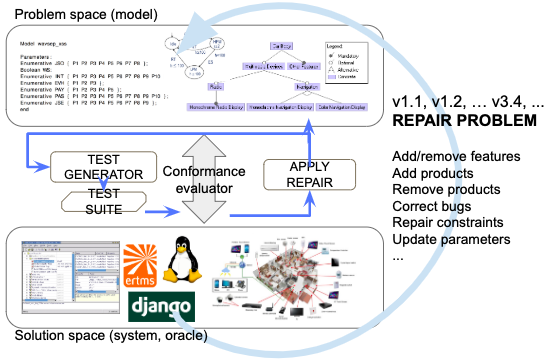
\includegraphics[width=.8\columnwidth]{images/repair.png}
	\caption{Test-Driven process to repair models}
	\label{fig:approach}
\end{figure}

%We plan to evaluate effectiveness and efficiency of the test-driven repair techniques on different applications, with real-world models and systems: from literature and from industrial cases. Apart from the already investigated applications to combinatorial and feature models, we plan to study a scenario of repair of 
%timed automata (TA), high order logic expressions, and finite state machines, for example. % they all have
%Timed automata are mainly used to describe the behavior of communication protocols, real-time systems and cyber-physical systems.
%The model could be abstracted to obtain parameters representing timing constraints in the guards or in the locations, resulting in a Parametric Timed Automata (PTA), and tests drive the detection of a configuration for such parameters, that reflects the \textit{updated} system.
%Each test, in this case, could be an \textit{execution trace}.%, that can happen or not in a given system, or according to the new specification.

%The dissemination plan consists in applying test-driven repair to real-world software systems, and possibly release tools, in addition to publishing papers to venues related to software testing or to the particular application for which test-driven repair has been applied.
%If real-world case studies coming from collaborations with industries in the sector are found, it would be an added value.


\part{Request-Driven Repair}
\chapter{Repair of Feature Models}
Feature models are a widely used modeling notation for variability management in software product line (SPL) engineering. 
%In order to keep an SPL and its feature model aligned, feature models must be changed by including/excluding new features and products, either because faults in the model are found or to reflect the normal evolution of the SPL.
%Such changes can be complex and error-prone due to the size of the feature model.
%Therefore, 
We developed an approach that \textit{repairs} a feature model w.r.t. a given update request in the form of combinations representing a set of configurations to be accepted or rejected, that may be detected by \textit{failing} test cases, or directly by engineer domain knowledge. % from a change in the specification.
The method is based on an evolutionary algorithm that iteratively mutates the original feature models and checks if the update request is semantically fulfilled.
We employ mutations such as switching an optional feature to mandatory, or changing an \emph{or} group to an \emph{and} group, based on \cite{arcaini2018evolutionary}.
% \cite{arcaini2018evolutionary,ARCAINI201964}.
We generate faults between two real versions of feature models of the {\tt MobileMedia}, {\tt HelpSystem},  {\tt SmartHome}, and {\tt ERP\_SPL} systems in the SPLOT repository\footnote{\url{http://52.32.1.180:8080/SPLOT/feature_model_repository.html}}, and we notice that although our approach does not guarantee to completely update all the possible feature models, on average, around 89\% of requested changes are applied, with minimal edits.%, helping in preserving domain knowledge.

%\subsection{Test generation and fault localization}
%The process is driven by update configurations or failure-inducing combinations in the input parameters of the system, and black-box (in particular, combinatorial) test generation and fault detection and localization techniques, are important to support engineers in determining such inputs for the repair process.
%To this purpose, we make use of a tool to make it easier the editing of combinatorial models, and the test suite generation, called CTWedge \cite{IWCTGargantini2018}, and we devise a fault localization process, based on combinatorial testing, that guarantees to find the correct detection of failure-inducing combinations, under the assumption that the maximum strength of the real failure-inducing combinations is known.

\part{Failure-Driven Repair}
\chapter{Repair of Configuration Constraints}
A model for a combinatorial problem consists of parameters which can take various domain values. Combinatorial models may have also constraints among parameter values to, for example, model inconsistencies between certain hardware components, limitations of the possible system configurations, or simply because of design choices \cite{gargantini_combinatorial_2017}.
%Some methods have been introduced to automate the process of inferring constraints, but they do not aim at \textit{repairing} existing ones \cite{abukwaik_extracting_2016,Temple:2016:UML:2934466.2934472}. 
%Therefore, in \cite{gargantini_combinatorial_2017}
The devised iterative approach uses a fault-localization tool based on combinatorial testing, called BEN \cite{ghandehari2018combinatorial}, and CIT policies introduced in \cite{Gargantini16:validation} to find failure-inducing combinations of parameter values.
The model is then repaired \textit{logically}, by translating such failure-inducing combinations into expressions in propositional logic.
The repairs are of two types, depending on whether the model is true and the system (i.e., the oracle) false for a given test case (in this case, the model is \textit{under-constrained}) or vice-versa (in this case, the model is \textit{over-constrained}). Tab. \ref{table:testsandfaults} reports possible scenarios in which such condition may occur in a system with three boolean parameters A, B, C, that map to directives in a C program in which both B and C can be enabled only if also A is activated.
\begin{table}[!tb]
	\caption{Test suites with faults (in gray)}\label{table:testsandfaults}
	\begin{comment}
	\begin{tabular}{c|c|c||c|c|c}
	A & B & C & oracle & \mfU & \mfO\\
	& & & $A \rightarrow B$,$ A \rightarrow C$ & $A \rightarrow B$ & $A \rightarrow B$,$C$\\
	\hline 
	T & T & T & T & T & T \\
	T & T & F & F & \cg T & F \\
	T & F & T & F & F & F \\
	F & T & T & T & T & T \\% & \underConstr fault\\
	F & T & F & T & T & \cg F\\
	F & F & T & T & T & T\\
	F & F & F & T & T & \cg F\\
	\end{tabular}
	\end{comment}
	\resizebox{.8\columnwidth}{!}{
		\begin{subtable}[t]{.5\columnwidth}
			\centering
			\caption{\underConstr fault}
			\label{table:underConstrFault}
			\begin{tabular}{c|c|c||c|c}
				A & B & C & \mfU & oracle\\
				\hline 
				T & T & F & \cg T & \cg F\\% & \underConstr fault\\
				T & F & F & F & F\\
			\end{tabular}
		\end{subtable}%
		\begin{subtable}[t]{.5\columnwidth}
			\centering
			\caption{\overConstr fault}
			\label{table:overConstrFault}
			\begin{tabular}{c|c|c||c|c}
				A & B & C & \mfO & oracle\\
				\hline 
				F & T & T & T & T\\
				F & F & T & T & T\\
				F & T & F & \cg F & \cg T\\% & \overConstr fault\\
				F & F & F & \cg F & \cg T\\% & \overConstr fault\\
			\end{tabular}
		\end{subtable}%
	}
\end{table}


Experiments for five real-world systems (Libssh, Telecom, Aircraft, Concurrency, and Django) show that our approach can repair on average 37\% of conformance faults. Moreover, we also notice that it can infer and repair parameter constraints for the configurations that lead to a successful startup of Django, a well-known open source web application framework written in Python.

%For test generation we used a framework called CTWedge

%\subsubsection{XSS Vulnerabilities Constraints}
%Combinatorial models are also suitable to model parts of XSS attack vectors, with a limited number of possible values.
%We applied our iterative approach also to such models, using as oracle a script that runs the web application under test, inject the attack vector in a particular input field in a form, and checks wether the injected Javascript code has been present in the response page.  We evaluated our approach empirically on four systems from the Web Application Vulnerability Scanner Evaluation Project (WAVSEP), and on two real-world web applications, obtaining an accurate model of the constraints among parameters that cause an attack vector to break the sanitization function of the system.

\section{Using Iterative Constraint Repair to Detect XSS Vulnerabilities}
\chapter{Repairing Timed Automata Clock Guards through Abstraction and Testing}

\part{Tools to Support Model Repair}
\chapter{CTWedge: Migrating Combinatorial Interaction Test Modeling and Generation to the Web}
Combinatorial Interaction Testing (CIT) is becoming a widespread practice for software testing.
The presence of tools for CIT is of fundamental importance because performing CIT activities manually can be error prone and time consuming. The site pairwise.org\footnote{See \url{http://www.pairwise.org/tools.asp}} lists at least 43 tools supporting several CIT activities while the paper~\cite{NieL11} reviewed the CIT literature and found around 20 tools. 
%
Most of the tools are classical programs or plugins of existing programs/platforms.  In all these cases, the user has to download, install, and execute the program on his/her machine.  Some tools offer a GUI interface, for example, for defining the models and run the test generation, while others rely on other programs for some activities (like PICTMaster, based on PICT~\cite{czerwonka_pairwise_2006}, that works entirely inside Microsoft Excel). %(like PICT~\cite{czerwonka_pairwise_2006} that gives the output as an Excel spreadsheet).
In~\cite{citlab12} we have presented a plugin for the eclipse IDE that helps the user in writing CIT models with constraints by leveraging all the expected features of a modern IDE, and it generates combinatorial test suites by using third party programs (like CASA or ACTS).

However, this classical approach poses some challenges. First, the user must install the chosen CIT tool, which in turn may require some dependencies, like java, or in case of plugin, it requires the installation of another program or application like eclipse, excel and so on. Then the user must use his/her machine for running the test generation algorithms. For experienced users with powerful machines they can administer, this is not a real problem. However, for novice users with not so powerful computer, or students that are just learning the CIT principles, or software developers using computer they cannot administer, this can become a cost to be considered and it may be an obstacle for the use of CIT.

Second, from the point of view of tool developers, the distribution of programs means that they have little or no control on the software once is installed: when a bug is discovered the developer has to fix the bug, publish a new version of the tool and hope that the users will update their software. Moreover, the developer has no idea about how the software is used: what are the typical scenarios of use (big or small models, for example), what are the features that are mostly used (for example, what modeling features are more used). Furthermore, it is difficult for tool developers to apply a cost model able to reward their effort in developing and deploying the CIT tool. Indeed, most of the tools are given away for free by researchers supported by their own organization.

A possible solution of these problems could be the offer of CIT features as software as a service (SaaS). SaaS is software that is accessed through Internet by using a classical web browser.  The SaaS software is actually hosted on the vendor’s servers, and the customers log in and perform tasks as necessary.  The 
vendor is the one who is ultimately responsible for hosting, upgrading and maintaining the program as needed.  There is an extensive literature about SaaS and the advantages (together with limitations) are well known~\cite{Menken:2008}. 

There are already experiences in using the web for CIT. For instance, CTWeb Classic~\cite{usaolaframework}, CTWeb Plus~\cite{ctwebplus}, TestCover~\cite{testcover}, Hexawise~\cite{hexawise}, and PairWiser~\cite{pairwiser}. 

However, as we will discuss in the related work section, each tool has its own specific language to define combinatorial models, with its own predefined output formats and a (limited) set of supported existing or in-house algorithms for test case generation. Not all those tools are equally powerful or easy to use, and many of them are commercial or require registration.

%However, as we will discuss in the related work section, they lack of some features: very limited editing capabilities, little support for constraints, test generation using in-house algorithms, and limited export formats.

For this reason, starting from our experience with \citlab~\cite{citlab12}, we have worked on a web based application that allows the user to write CIT models in a similar way he/she would do in a classical IDE and it offers test suite generation by means of   server using known and community evaluated test generation algorithms. 
Our system, called \ctwedge (Combinatorial Testing Web EDiting and GEneration), introduces a rich language for combinatorial models, offers a powerful web editor, and allows the user to generate the CIT test suites on a server. The only software needed to use \ctwedge is a modern web browser.

The paper is organized as follows. In Sect. \ref{sec:language} we present the modeling language (in an abstract way) we use to define CIT models. In Sect. \ref{sec:ctwedge} we introduce our tool, its architecture, its web editing capabilities, and the generator engine. A detailed comparison with other similar web based tools is presented in  Sect. \ref{sec:related}. Future works and possible directions of extension are presented in Sect. \ref{sec:futurework}. Sect. \ref{sec:conclusions} concludes the paper.


\section{A simple language for CIT models}\label{sec:language}

We have devised a simple textual language for CIT models which is suitable to be used in web editors. It allows the definition of parameters, each with its name and (finite) domain, and it is based on our previous language defined for \citlab \cite{citlab12}. We allow the following parameter types: 

\begin{enumerate}
	\item \textsf{Boolean} with only two possible values \textsf{true} and \textsf{false}
	\red{ (all lower or all upper case).}
	%(which can be written also all uppercase). 
	The two boolean constants are \red{ also }considered of Boolean type.
	\item \textsf{Ranges} that are integer intervals defined by their lower bound $l$ and upper bound $u$. With $[l..u]$ we denote all the integers between $l$ and $u$ included.
	\item \textsf{Enumerative} that are a list of possible values between \{\}. We are rather liberal about the elements and we allow identifier starting also with a number, natural numbers, and strings. For example, one could define a  enumerative \textsf{values} in this way:
	\begin{lstlisting}[language=ctwedge]
	values : {100, 1M, "my name", cit}
	\end{lstlisting}
\end{enumerate}

A simple example of combinatorial model with three parameters is shown in Fig. \ref{fig:ctexample}. 

\begin{figure}[tb]
	\centering
	\begin{lstlisting}[language=ctwedge,frame= single]
	Model Phone
	Parameters:
	emailViewer : Boolean
	textLines:  [ 25 .. 30 ]
	display : {16MC, 8MC, BW}
	\end{lstlisting}
	\caption{A smartphone example}
	\label{fig:ctexample}
\end{figure}

There are some semantic rules about the parameters and their definitions, defined as follows:
\begin{enumerate}
	\item The name of each parameter must be unique.
	\item In \textsf{Ranges}, the lower bound $l$ must be less than the upper bound $u$.
	\item The elements in each \textsf{Enumerative} must be distinct. We allow two enumerative parameters to share some elements, though.
\end{enumerate}


\subsection{Constraints}

A distinctive feature of our langauge is the support of modeling constraints among parameters. 
In most configurable systems, constraints or dependencies exist between
parameters. Constraints may be introduced for several reasons, for example, to
model inconsistencies between certain hardware components, limitations of the
possible system configurations, or simply design choices~\cite{CohenISSTA07}.
In our approach, tests that
do not satisfy the constraints are considered \emph{invalid} and do not need to
be produced. For this reason, the presence of constraints may reduce the number
of tests of the final test suite (but it may also increase it
~\cite{CohenISSTA07}). However, the generation of tests considering constraints
is generally more challenging than the generation without them, and several test generation techniques still do not support constraints, at least not in a direct manner. In \ctwedge we decided to focus more on techniques supporting constraints.

In \ctwedge, we adopt the language of propositional logic (with the usual logical operators) with equality and arithmetic to express constraints. To be more precise, we use propositional calculus, enriched by the arithmetic over the integers and enumerative symbols. As operators, we admit the use of equality and inequality for any variable, the usual Boolean operators for Boolean terms, and the relational and arithmetic operators for numeric terms. To be more precise, Table \ref{tab:validity} reports all the rules we have defined to check if a constraint is semantically correct.

\begin{table*}
	\centering
	\begin{tabular}{|l|l|l|}
		\hline 
		\textbf{Expression}	& \textbf{Case} & \textbf{Correct iff}\\\hline
		\multirow{7}{*}{\shortstack{$e_1\ op\ e_2$	with $op \in \{=, \neq \}$ $\rightarrow boolean$ \\ $ e_2\ op\ e_1$ with $op \in \{=, \neq \}$ $ \rightarrow boolean$ }}  & $e_1$ enumerative, $e_2$ element& $e_2$ belongs to $e_1$ elements \\\cline{2-3}
		
		& $e_1$ enumerative, $e_2$  enumerative& $e_1$ and $e_2$ share at least one element \\\cline{2-3} 
		&  $e_1$ range, $e_2$ range & $e_1$ and $e_2$ share at least one number \\\cline{2-3}
		& $e_1$ range, $e_2$ number & always \\\cline{2-3}
		& $e_1$ number, $e_2$ number & always \\\cline{2-3}
		& $e_1$ boolean, $e_2$ boolean & always\\\cline{2-3}
		%& $e_1$ boolean, $e_2$ boolean constant & always \\\cline{2-3}
		\hline 
		
		\multirow{3}{*}{\shortstack{$e_1\ op\ e_2$	with $op \in \{<, \le, >, \ge \}$ $\rightarrow boolean$ \\ $ e_2\ op\ e_1$ with $op \in \{<, \le, >, \ge \}$ $ \rightarrow boolean$ }}  &  $e_1$ range, $e_2$ range & $e_1$ and $e_2$ share at least one number \\\cline{2-3}
		& $e_1$ range, $e_2$ number & always \\\cline{2-3}
		& $e_1$ number, $e_2$ number & always \\\cline{2-3}
		%& $e_1$ boolean, $e_2$ boolean & always \red{sicuro???}\\\cline{2-3}
		%& $e_1$ boolean, $e_2$ boolean constant & always \\\cline{2-3}
		\hline 
		
		\multirow{3}{*}{\shortstack{$e_1\ op\ e_2$	with $op \in \{\wedge, \vee, \rightarrow\}$ $\rightarrow boolean$ \\ $ e_2\ op\ e_1$ with $op \in \{ \wedge, \vee, \rightarrow \}$ $ \rightarrow boolean$ }}  & \multirow{3}{*}{$e_1$ boolean, $e_2$ boolean} & \multirow{3}{*}{always} \\ %\cline{2-3}
		& & \\
		& & \\ 
		
		%& $e_1$ boolean, $e_2$  boolean constant & always \\\cline{2-3} 
		%& $e_1$ not a boolean or $e_2$ not a boolean & never \red{skip?} \\\cline{2-3}
		\hline
		
		%\multirow{2}{*}{\shortstack{$e$ $ \rightarrow boolean$ \\ $\neg e$ $ \rightarrow boolean$ }}  & $e$ boolean & always \\\cline{2-3}
		%& $e$ boolean constant & always \\\cline{2-3} 
		%\hline
		
		\multirow{1}{*}{$\neg e$ $ \rightarrow boolean$}  & $e$ boolean & always \\\cline{2-3}
		%& $e$ boolean constant & always \\\cline{2-3} 
		%& $e$ not a boolean& never\\\cline{2-3} 
		\hline
		
		\multirow{4}{*}{$e_1\ op\ e_2$	with $op \in \{+, -, *, /, \%\}$ $\rightarrow number$}  & $e_1$ number, $e_2$ number & $e_2 \neq 0$ if $op=/$ or $op=\%$ \\\cline{2-3}
		& $e_1$ range, $e_2$  range & always \\\cline{2-3} 
		&  $e_1$ range, $e_2$ number & $e_2 \neq 0$ if $op=/$ or $op=\%$ \\\cline{2-3}
		&  $e_1$ number, $e_2$ range & always \\\cline{2-3}
		\hline
	\end{tabular} 
	\caption{Rules of \ctwedge Language Validator for Constraints}\label{tab:validity}
\end{table*}

For example, we can write constraints in this way:

\begin{lstlisting}[language=ctwedge,frame= single]
Model Phone
..
Constraints:
# emailViewer => textLines > 28 #
# emailViewer and display != 16MC => textLines > 28 + 3#
\end{lstlisting}

Many test suite generation tools provide a limited support for constraints. For instance, AETG \cite{605761,Lott:2005:MRC:1083274.1083281} allows only simple constraints of type \textsf{if then else} or \textsf{requires}. The language of \ctwedge is in this aspect more expressive, as it is targeted to be more general than existing tools. In the specific case of AETG, the translation of those templates into our logic is straightforward. For example the \textsf{if then else} constraint can be translated by two implications.
Other tools \cite{CohenISSTA07} allow constraints only in the form of forbidden combinations \cite{Golumbic:2011:GTC:2028636}. Our language is more general, as a forbidden tuple would be translated as a \textit{not} statement. For instance, a forbidden pair \textsf{emailViewer = false; display = 16MC} would be represented by the following constraint:
$$\textsf{\#\ not\ (emailViewer = false\ and\ display = 16MC)\ \#}$$
However, the explicit list of the forbidden combinations may explode and it may become impractical and error-prone to represent it. For example, if the model of mobile phones presented in Fig. 1 had a constraint that

\emph{"A front video camera requires also a 16MC display"}. This constraint would be translated into two forbidden tuples:

$$\textsf{(emailViewer = true, display = 8MC);}$$
$$\textsf{(emailViewer = true, display = BW);}$$
However, the translation as constraint in general form would be simply:
$$\textsf{\#\ emailViewer =\textgreater\ display = 16MC\ \#}$$
which is more compact and more similar to the informal requirement.

In our language semantics, a test case is valid only if it does not contradict any constraint in the specification. Others \cite{BRYCE2006960} distinguish between combinations to be avoided \textit{if possible} (soft constraints), and the forbidden combinations (hard constraints), which must always be avoided (our case). %We consider only hard constraints, for now.

Other tools, like CASA \cite{CASA}, support only constraints in conjunctive normal form, without arithmetic or relational operators.


\subsection{Xtext}

There are countless ways to define a language together with its parser. One emerging technique for Domain Specific Language modeling is the use of Xtext~\cite{Eysholdt:2010}. By defining the grammar of the DSL of choice by means of a Xtext grammar, the language designer obtains a parser, APIs to programmatically access models, a serializer and a smart editor for it. The editor provides many features out-of-the-box, such as syntax highlighting, content-assist, folding, jump-to-declaration and reverse-reference lookup across multiple files.  We had already used Xtext for defining the language in \citlab~\cite{citlab12}. Xtext support also the generation of a web editor, as we present in the following section.

Grammar rules written in Xtext are very close to the standard (E)BNF production rules. For instance, the main grammar rule that defines the whole CIT model is defined as follows:

% uso matlab per via delle single quote
\begin{lstlisting}[language=Matlab,columns=fullflexible,basicstyle=\small\ttfamily,stringstyle=\ttfamily\color{blue},upquote=true]  
CitModel:
'Model' name=ID 
'Parameters' ':' (parameters+=Parameter)+ 
('Constraints' ':' (constraints+=Constraint)+)?
\end{lstlisting}

Xtext can display the production rules by means of syntax diagrams, also known as railroad diagrams. For example, the rule presented before for {\small\ttfamily CitModel} is shown in Fig. \ref{fig:grammarrule}.

\begin{figure}
	\centering
	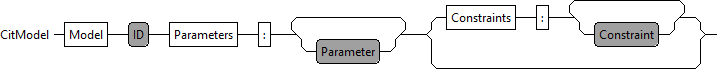
\includegraphics[width=1\linewidth]{images/grammar_rule}
	\caption{{\small\ttfamily CitModel} rule diagram}
	\label{fig:grammarrule}
\end{figure}

Because Xtext is based on ANTLR, it does not allow left recursive parser rules and parsing nested expressions is not as simple as writing a EBNF rule. The \ctwedge language parses the constraints by defining the precedence among operators implicitly by left-factoring expression definitions. For example, in order to parse the AND operators before the OR operators,  \ctwedge  introduces the following two rules that are not left recursive:

\begin{lstlisting}[language=Matlab,columns=fullflexible,basicstyle=\small\ttfamily,stringstyle=\ttfamily\color{blue},upquote=true,morekeywords={returns}]  
OrExpression returns Expression:
AndExpression ({OrExpression.left=current} 
OR_OPERATOR (right=AndExpression))*;

AndExpression returns Expression:
EqualExpression ({AndExpression.left=current}
AND_OPERATOR (right=EqualExpression))*;
\end{lstlisting}



The definitions of semantic constraints in Xtext is performed by user-defined validator classes written in Java or in Xtend containing methods annotated by {\small\ttfamily @Check}. For instance, to check that in the definition of any range domain of our CIT models  the upper bound is greater than the lower bound, we have introduced the following checking method:

\begin{lstlisting}[language=Java,morekeywords={def},basicstyle=\small\ttfamily]
@Check
def checkRangeIsCorrect(Range range) {
if (range.getBegin() >= range.getEnd())
error("The second term must be greater ...");
}
\end{lstlisting}

\section{\ctwedge: CT Web Editor and Generator}\label{sec:ctwedge}

In this section, we present our tool \ctwedge. 
As we can see in Fig.~\ref{fig:architecture}, the tool is composed by a language definition component (with its Xtext parser and validator), a web-based editor for the \ctwedge language, with some options for test generation and a test suite visualizer and exporter, and a test suite generator that exploits third-party test generation tools.

The tool is written in Java and Xtext, and can be deployed on any Web-application server, such as Apache Tomcat. It is publicly available at: \url{http://foselab.unibg.it/ctwedge/}.



\begin{figure}[bt!]
	\centering
	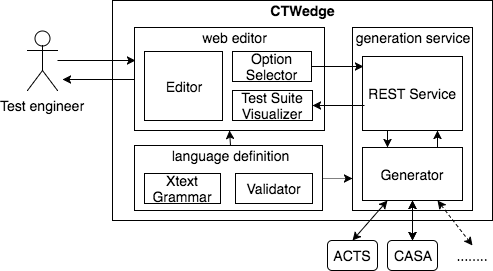
\includegraphics[width=\columnwidth]{images/architecture.png}
	\caption{\ctwedge architecture}\label{fig:architecture}
\end{figure}



%\section{CTWedge: Combinatorial Testing Web Editor and GEnarator}
\subsection{Combinatorial Testing Web Editor}
%\subsection{Editing}

In order to implement a web-based editor, we can leverage the Xtext framework, since Xtext starting from version 2.9 offers an interface for integration of text editors in web applications. The text editors are implemented in JavaScript, and language-related services such as code completion are realized through HTTP requests to a server-side component.

The Xtext web-based editor provides several features, like content assist to help the user to complete the models, validation to check the correctness, syntax coloring, and formatting.

The \ctwedge web editor is based on Ace (Ajax.org Cloud9 Editor)\footnote{See \url{https://ace.c9.io/}}, but other web editors (like Orion and CodeMirror) are available. Xtext does not yet provide support for the recently standardized Language Server Protocol
%\footnote{See \url{https://github.com/Microsoft/language-server-protocol}}
\cite{lsp}, which we plan to include in our tool as a future work.  A screenshot of the \ctwedge web editor is shown in Fig. \ref{fig:editor}. The web editor provides an immediate feedback while writing by means of syntax highlighting, auto completion, and errors markings. 

The validation of the model is performed run-time while the user writes it. If the validator finds an error in the model, it generates an error message. The nature of the error is indicated in the pop-up box appearing when positioning the cursor over the error sign, and the point in which the error occurs is marked in the editor. Fig. \ref{fig:validation} shows how model validation errors are displayed to the test engineer.



\begin{figure*}[bt!]
	\centering
	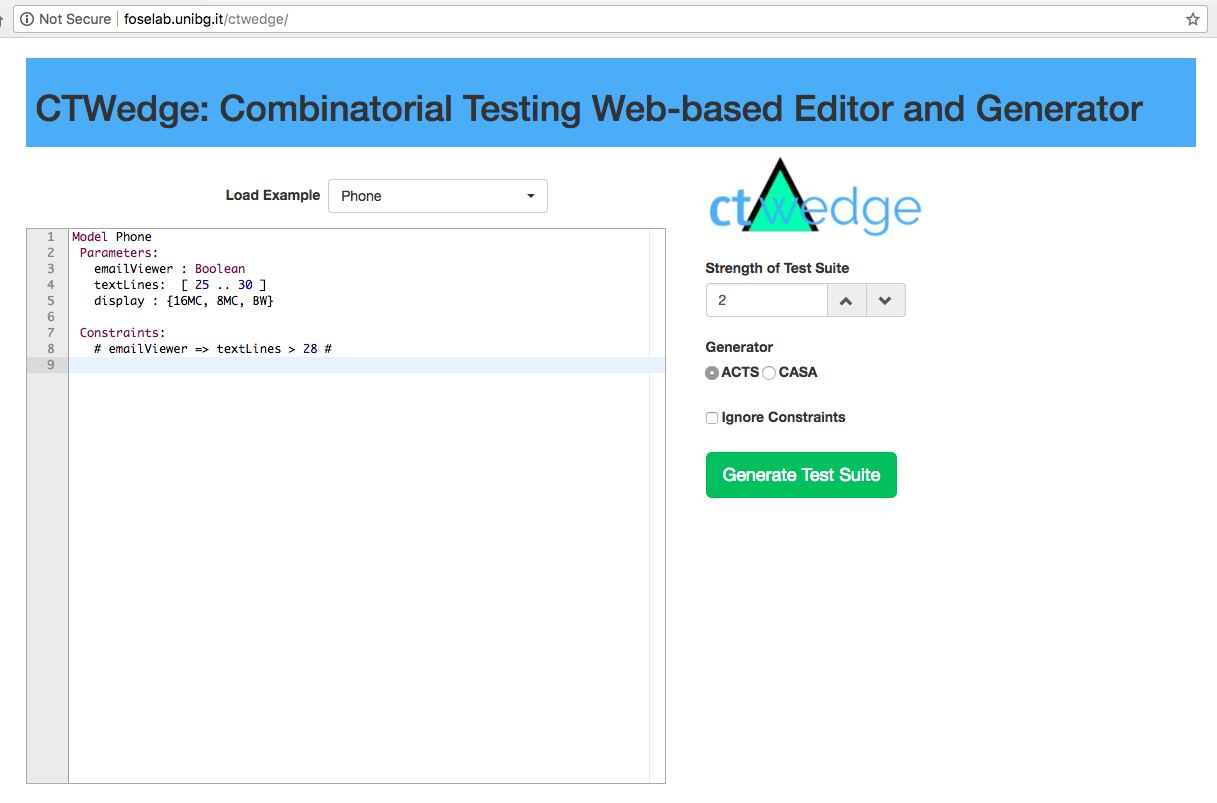
\includegraphics[width=\textwidth,trim={0 10cm 0 0},clip]{images/editor2.png}
	\caption{\ctwedge web editor}\label{fig:editor}
\end{figure*}

The editor allows to load predefined examples of combinatorial models, selected from literature \cite{segall_using_2011} and converted into \ctwedge language format (with extension \textit{.ctw}).

\red{Graphical components (buttons and option selectors) are built using the JavaScript frameworks JQuery}\footnote{JQuery: \url{https://jquery.com/}} 
and Bootstrap\footnote{Bootstrap: \url{https://getbootstrap.com/}}.
\red{ The web application is fully compatible also with mobile devices (Android and iOS), from any recent Web browser with JavaScript enabled.}

%\red{screenshot validazione per face vedere che l'editor mostra errori. MARCO}

\begin{figure}[bt!]
	\begin{subfigure}{\columnwidth}
		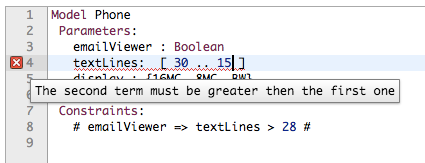
\includegraphics[width=.8\columnwidth]{images/validation1.png}\caption{Validation of Range parameter}
	\end{subfigure}
	
	\begin{subfigure}{\columnwidth}
		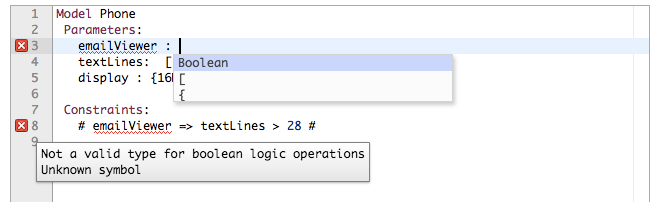
\includegraphics[width=\columnwidth]{images/validation2.png}\caption{Code recommender. Unknown symbol error.}
	\end{subfigure}
	
	\begin{subfigure}{\columnwidth}
		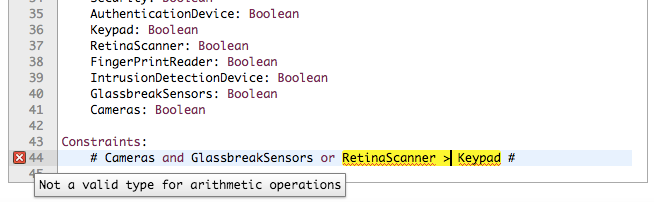
\includegraphics[width=1\columnwidth]{images/validation3.png}\caption{Validation of relational operations}
	\end{subfigure}
	\caption{Examples of \ctwedge validation errors}\label{fig:validation}
\end{figure}


\subsection{Test generator web service}

%\red{cosa is questo modulo}

The function of actually generating a test suite from the test model and option parameter is web-served and performed by the test generation service which is the component of \ctwedge.
The test generation service is composed by two modules: a REST\footnote{REST: Representational State Transfer} service and a language translator.

The REST service handles input model and option parameters for the generation, calls the generators from which it gets back the tests and it is responsible to deliver them to the web browser. 

The test generator acts as a \textit{driver} between \ctwedge and the various third party combinatorial test generation tools, which are usually accessible via their own APIs, or via command line. The test generator exports the combinatorial model along with the generator options, into the the specific language of the external tool, or directly into the tool's APIs. Then, it waits for the generator to compute the test suite, and once ready, it passes it back to the REST service. If necessary, the generator also maps any parameter values back to the original \ctwedge model format. Each external program needs its own translator.

\begin{table}[!tb]
	\caption{Request parameters to \ctwedge generation service}
	\centering
	\resizebox{0.5\textwidth}{!}{%
		\centering
		\begin{tabular}{l l p{2.55cm} p{3.35cm}}
			\toprule
			\textbf{Parameter} & \textbf{type} & \textbf{description} & \textbf{values} \\
			\midrule
			model & String & the combinatorial model & as written and validated by the editor (see Sec. \ref{sec:language}) \\ 
			strength & Int & the combinatorial interaction strength & any integer above 1 (default is 2: pairwise) \\ 
			generator & Enum & the tool to be used & ["acts", "casa"] (so far) \\
			ignConstr & Boolean & if constraints should be ignored in test generation & ["true", "false"] (default is false) \\ 
			\bottomrule
		\end{tabular}
	}
	\label{tab:parameters}
\end{table}

The REST service accepts an HTTP GET or POST request with parameters as described in Tab. \ref{tab:parameters}.
For sake of brevity, an example URL request to the web generator service is shown in Fig. \ref{fig:urlexample}.

\begin{figure}[tb!] % https://tex.stackexchange.com/questions/116534/lstlisting-line-wrapping
	\centering
	\lstset{
		basicstyle=\ttfamily\small,
		columns=fullflexible,
		frame=single,
		breaklines=true,
		postbreak=\mbox{\textcolor{red}{$\hookrightarrow$}\space},
		language=url
	}
	\begin{lstlisting}
	http://foselab.unibg.it/ctwedge.generator?model=Model%20Phone%20Parameter:%20...>28%20#&strength=2&generator=acts&ignConstr=false	
	\end{lstlisting}
	\caption{Generator URL example}
	\label{fig:urlexample}
\end{figure}

So far, we interfaced \ctwedge with ACTS~\cite{ACTS} and CASA~\cite{CASA}. ACTS is accessed  via it internal APIs whereas CASA is called via command line.

The resulting test suite is returned in CSV\footnote{CSV: Comma Separated Values} format. The header line contains the parameter names, and each following line represents a single test, with parameter values.
%\red{Note that for coverage evaluation, the first line with the parameter names may need to later be removed, in order to not miscalculate coverage.}
The web front-end allows to download CSV file to further local use, and shows the test suite in the browser by converting it into an HTML table. Conversion is straightforward and done client-side via Javascript.

Arithmetic operations and relational operators ($>$, $<$, $\le$, $\ge$) are not natively supported by CASA, and in presence of such constraints, an error is reported to the user, as in Fig. \ref{fig:casaError}.
% \red{aggiungere errore CASA?}

\begin{figure}[bt!]
	\centering
	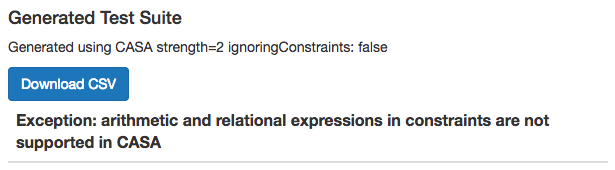
\includegraphics[width=\columnwidth]{images/casaError.png}
	\caption{Message of operations not supported in constraints for CASA generator tool}\label{fig:casaError}
\end{figure}

\begin{figure}[bt!]
	\centering
	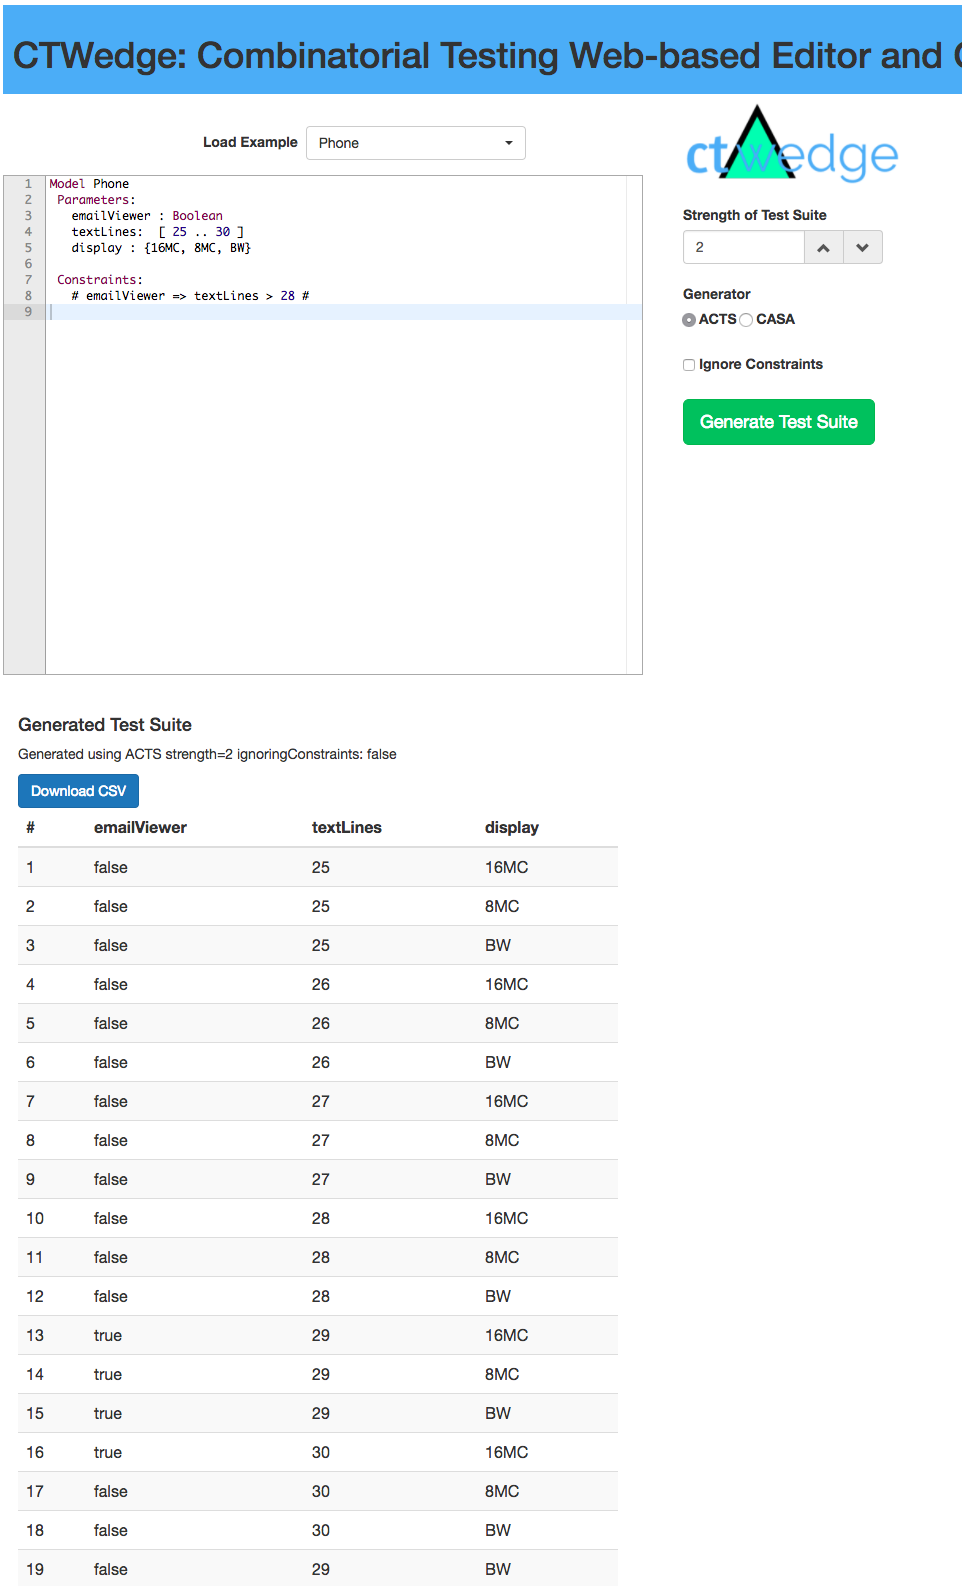
\includegraphics[width=\columnwidth,trim={0 0 7cm 0},clip]{images/generatedTable.png}
	\caption{\ctwedge visualization of the generated test suite}\label{fig:generated}
\end{figure}

The HTML table showing the generated test cases is located below the editor on the same window. This location is less invasive than a brand new tab as it does not hide or replace the current combinatorial model in the editor. Despite it is not immediately visible to the user, who may think the output is hidden, we believe that it preserving the access to the current screen is the most important aspect to be preserved.

The generator is called by the editor by AJAX, with an asynchronous XmlHttpRequest.




A screenshot of how the generated test suite is presented to the user is shown in Fig. \ref{fig:generated}. 
It is shown as plain HTML table, with the possibility to download the data as CSV. %\red{considerare ideaa di mettere tabella sotto con indice - MARCO} \blue{updated screenshot}
%\red{da mettere errore per alcuni constraint usando CASA}




%\subsection{Test generation}

\section{Related Work}\label{sec:related}



With the success of the SaaS pattern, web-based tools have rapidly gained popularity due to their portability and ease of use. There exist some web-based services also for combinatorial test case generation, each with its own peculiarities. SaaS tools, however, still represents a small number of all the available tools for test case generation: IDE plugins and desktop applications represent almost the totality of the current tools. We looked for tools from the pairwise.org\footnote{See \url{http://www.pairwise.org/tools.asp}} and softwaretesters.net\footnote{See \url{https://softwaretesters.net/zbxe/index.php?mid=downloadtool&category=4258006&sort_index=readed_count&order_type=desc}} tool catalogs, and from the web, to the best of our searching skills. 


\begin{table}[bt!]
	\centering
	\setlength\tabcolsep{2pt}
	\begin{tabular}{l P{52mm} P{52mm}}
		Tool & URL & Documentation \\
		\toprule
		TestCover & \url{https://testcover.com} & \url{https://testcover.com/sub/instructions.php} (visible after registration) \\
		\midrule
		CTWebClassic & \url{http://alarcostest.esi.uclm.es/CombTestWeb/combinatorial.jsp} & \url{http://alarcostest.esi.uclm.es/CombTestWeb/stuff/usersManual.pdf} \\
		\midrule
		CTWebPlus & \url{http://www.testcasegeneration.com} or \url{http://www.ctwebplus.com/} & \url{http://www.ctwebplus.com/stuff/userManual.pdf} \\
		\midrule
		HexaWise & \url{https://hexawise.com/} & \url{https://hexawise.com/Hexawise_Introduction.pdf} \\
		\midrule
		PairWiser & \url{https://inductive.no/pairwiser/} & \url{https://inductive.no/pairwiser/knowledge-base/} \\
		\bottomrule
	\end{tabular}\caption{Tool resource links}\label{tab:docs}
\end{table}

We compare the following five SaaS for CIT, listed in Tab. \ref{tab:docs}:
\begin{itemize}
	\item TestCover~\cite{testcover} is a commercial web-based combinatorial test case generator supported by Testcover.com, LLC, founded in 2003. The tool was also presented at IWCT 2016~\cite{sherwood2016embedded}.
	\item CTWeb Classic~\cite{usaolaframework} is a free online tool for combinatorial testing and state machine test case generation,  developed at University of Castilla-La Mancha (Spain).
	\item CTWeb Plus~\cite{ctwebplus}, an academic combinatorial test generation tool developed as improvement of CTWeb Classic. CTWeb Plus is now commercially supported.
	\item HexaWise~\cite{hexawise}, a commercial combinatorial test case editor and generator, launched in 2009 by Hexawise, Inc.
	%\item PairWiser~\cite{pairwiser}, a free web-based tool provided by Inductive AS. It will be shut down January 15th, 2018, replaced by a desktop, standalone application.
	\item PairWiser~\cite{pairwiser}, a \red{commercial web-based tool provided by Inductive AS. The online version was shut down January 15th, 2018. After that date, only the standalone application, for own-server installation, is available.}
\end{itemize}

%shown in Tab. \ref{tab:comparison}

\red{All tools are well documented, with examples and tutorials. Links of on-line editors and official documentation resources of these tools are shown in Tab. \ref{tab:docs}}
%Documentation about how to input a combinatorial model is not rich in many of the tools, which provide only a limited set of examples to copy/paste, or to load into the graphical interface, whereas \ctwedge also provides the language grammar definition.

%Very few of them have editor-support, either on-line or off-line, and even the only tool with a web-based editor, has no highlighting nor recommendation support.

%All of the 4 compared web-based tools are present in the pairwise.org list of CIT tools, in which, however, plugins and desktop tools represents almost the totality of the available tools.

\begin{table*}[bt!]
	\resizebox{\textwidth}{!}{%
	\centering
	\setlength\tabcolsep{2pt}
	\begin{tabular}{p{1mm}lP{24mm}P{24mm}P{24mm}P{24mm}P{24mm}P{24mm}}
		\hline
		& & \centering\textbf{TestCover}~\cite{testcover} & \centering\textbf{CTWeb Classic}~\cite{usaolaframework} & \centering\textbf{CTWeb Plus}~\cite{ctwebplus} & \centering\textbf{HexaWise}~\cite{hexawise} & \centering\textbf{PairWiser}~\cite{pairwiser} & {\textbf{\centering \ctwedge}} \\\toprule
		%& \textbf{URL}  & \textbf{Editing} & \textbf{Generation} &  \textbf{other infor}\\ 
		\hline 
		%URL & TestCover \url{http://testcover.com} & \url{http://www.testcasegeneration.com/} & \url{https://hexawise.com/} &  \url{https://inductive.no/pairwiser/} \\ 
		\multicolumn{2}{l}{\textbf{Language}} & & & & & & \\ 	
		%Enumeratives & & & & & \\
		%\red{Input type} & single text area & single text area & wizard process & wizard process & single text area \\
		%	\red{\shortstack{Define parameter values\\as range}} & \xmark & \xmark & \xmark & \xmark & \cmark \\
		&	Parameter Definition & Enumerative & Enumerative & Enumerative & Enumerative, Ranges (via value expansion) & Enumerative & Boolean, Enumerative, Ranges \\\midrule
		&	Constraints format & in DPB notation: via \emph{blocks} (i.e., sets of allowed combinations) & as \emph{if-then-else} & AND, OR, Else operators, not nested & invalid pairs (\emph{if..then..}) & guided by select boxes with rich choice of operators & arbitrary formula \\\midrule
		
		&	Numeric operators & \cmark (in PHP functions) & \xmark & \cmark & \cmark & \xmark & \cmark \\\midrule
		
		&	State Machine support & \cmark & \cmark & \cmark & \xmark & \xmark & \xmark \\\toprule % when they support Abstract State Machines
		%Verbosity & &  & high (GUI based) & & low \\\midrule
		%	Documentation & description, examples & examples & video tutorial & tutorial, examples & language grammar, examples \\
		\textbf{Editing} & & & & & & \\
		&	Web-based editor & text area & text fields and buttons + file upload & text fields, buttons, drawing area & text fields and buttons & text fields and buttons & text area \\\midrule
		&	Model Import/Export	& \cmark (Copy\&Paste as text) & \cmark & \xmark & \xmark & \xmark & \cmark   (Copy\&Paste as text)\\\midrule	
		&	Helping facilities & \xmark & button-guided (no facilities to build input file to upload) & button-guided & button-guided & button-guided & content-assist, syntax highlight, in-line error reporting \\\midrule 
		%Content Assist & \xmark & \xmark & \xmark & \xmark & \cmark \\\midrule 
		%		\red{REMOVE: LSP} & \xmark & \xmark & \xmark & \xmark & \xmark & \xmark \\\midrule
		&	Example Models & \cmark & \cmark & to be rebuilt from documentation file, not one-click loadable & \cmark & in the documentation & \cmark \\\toprule
		
		\multicolumn{2}{l}{\textbf{Generation}} & & & &  & & \\\midrule 
		&	n-wise & pairwise & pairwise & pairwise & up to 6-way interaction + mixed strength & up to 3-way interaction + mixed strength & \cmark \\\midrule
		&	Supported generators & All-pairs & AETG, PROW, All combinations, Each choice, Random, Bacteriologic & AETG, Pairwise, All-combinations, Each-choice, Comb, Random & not specified & not specified & ACTS, CASA \\\midrule
		%Random test generation & \xmark & \cmark & \xmark & \xmark & \xmark \\\midrule
		&	Export formats & HTML, WSDL interface & HTML, CSV & HTML & HTML, Excel, CSV, OPML & Excel, Jira issues & CSV, HTML \\\midrule
		&	Generate test scripts & \cmark (for Selenium) & \cmark (custom) & \cmark (custom) & \xmark & \cmark (custom) & \xmark \\\midrule
		&	Coverage visualization & \cmark & \xmark & \xmark & \cmark & \cmark & \xmark \\\toprule 
		\multicolumn{2}{l}{\textbf{Other information}} & & & & & & \\\midrule
		&	License & Commercial & Free & Commercial & Commercial & Commercial & Free \\\midrule
		&	Registration & subscription required &  optional & subscription required & subscription required & own-server installation & \xmark \\\midrule
		&	Online storage & \cmark & \xmark & \cmark & \cmark & \cmark (on own server) &\xmark  \\\midrule
		&	Additional notes & Functions in PHP into constraints. Also accessible via WSDL interface. %\red{TOREMOVE: Outputs also the number of pairs remaining uncovered after each test} 
		& Registration required for models with more than 5 parameters & Features a drawing area to represent states and transition of a state machine. The combinatorial model must be in the form of a state machine. & Has also a chart showing the interaction coverage after each test & Pairwiser online was shut down January 15, 2018. Available only for own-server installation. Allows to specify combinations to include in test suite. & -- \\\bottomrule 
		%URL & & \url{http://alarcostest.esi.uclm.es/CombTestWeb/combinatorial.jsp} &  \url{http://www.testcasegeneration.com} and \url{http://www.ctwebplus.com/}  & & & \\\midrule
		%Documentation & & \url{http://alarcostest.esi.uclm.es/CombTestWeb/stuff/usersManual.pdf} & \url{http://www.ctwebplus.com/stuff/userManual.pdf} & & \url{https://testcover.com/sub/instructions.php} (accessible via registration) & \\\midrule
	\end{tabular}
	}
	\caption{A comparison with other SaaS for CT}\label{tab:comparison}
\end{table*}

\red{To compare the SaaS tools among them and w.r.t. \ctwedge, we consider the following aspects, that we believe to be among the most relevant for a test engineer interested in using a web-based combinatorial test generation tool:}

\begin{itemize}
	\item \textbf{Language}. We look into the expressiveness of the accepted format for the combinatorial model in input. This evaluation includes:
	\begin{itemize}
		\item Parameter definition: how the parameter types and values  can be defined. For instance, a tool may support Boolean parameters or ranges of integers to express an enumerative made of all integers between two numbers. %, or Strings.
		\item Constraint format: if the constraints can be expressed as free combinations of logical and arithmetic operations among parameters, or have special formats, such as a set of forbidden tuples, a set of implications, or a set of if-then-else conditions. 
		%\item Functions: if generic, user-defined functions over parameters in the model, are allowed in the constraints.
		\item Numeric Operations: if constant numbers and basic numeric operations (+, -, *, /) are allowed in the constraints and/or in the generated code of test cases.
		\item State Machine support: if the language supports an easy input of state machines, to generate combinatorial tests for their execution.
	\end{itemize} 
	\item \textbf{Editing}. We evaluate how simple is for the test-engineer to input the combinatorial model into the tool. This category includes the following aspects:
	\begin{itemize}
		\item Web-based editor structure: how is the GUI of the web editor for writing the combinatorial model to be given in input to the tool; for example, if it is made by a single text area, or some buttons and text fields. Some tools use a single text area for the whole model, whereas some other tools use text inputs for individual parameters, reducing the need for parsing and text-highlighting.
		
		\item Import and export models: how the models can be exported to the file system and imported. For example, a tool may allow importing a text file written with another editor.
		
		\item Helping facilities: how the test engineer is guided in the input of the model in the web editor; for example with syntax highlighting, content assist, in-line error reporting, warning messages, or single text input fields to fill, and self-explanatory buttons to click.
		%		\item \red{TOREMOVE: LSP: If the back-end of the editor provides an API compatible with the Language Server Protocol standard, to make it easily extensible for usage with other tools.}
		\item Predefined example models: if there are examples of combinatorial models that can be easily loaded into the tool and executed to generate a test suite.
	\end{itemize} 
	\item \textbf{Generation}. We evaluate how the test suite generation is performed and how the output is presented to the user. This category includes the following aspects:
	\begin{itemize}
		\item n-wise: which interaction strengths of the generated test suite are allowed
		\item supported generators: which existing combinatorial test generation algorithms are supported
		\item export formats: in which formats the output is made available to the test-engineer
		\item Test-script generation: if there is a mechanism to allow the generated test vectors to be directly inserted into test cases written in custom code.
		\item Coverage visualization: if there is indication (textual or with charts) of the coverage reached after the execution of each test in the generated test suite.
	\end{itemize} 
	\item \textbf{Other information}. We consider aspects about the accessibility of the tool, and related features. We look the following aspects
	\begin{itemize}
		\item License: if commercial, free, or open source.
		\item Registration: if it is mandatory, optional or not made available.
		\item Online storage: if any data (input models, or output test suites) can be stored online.
		\item Additional notes: any other additional information that we consider worth being noted.
	\end{itemize} 
\end{itemize}



%Concerning language and editor support, HexaWise and PairWiser feature a completely graphical-based composer of combinatorial model: they do not allow scripting nor they feature a script editor. Input is only possible through buttons and text fields. Although this approach has the advantage of a quicker learning curve, it lacks all the features of a textual language, i.e., speed of writing and editing models, portability (possibility to edit and save models off-line or with other tools), expressiveness.


Table \ref{tab:comparison} compares the five tools and \ctwedge according to all these aspects.

\red{Concerning the web editor, while TestCover uses, as \ctwedge, a single text area for combinatorial model input,  all the others (CTWeb Classic, CTWeb Plus, HexaWise and PairWiser) feature a composer of combinatorial model guided by multiple selectors, text fields, and buttons. This approach of using buttons and text input fields, has the advantage of a quicker learning curve, and it does not need a language grammar, nor a parser, nor the helping facilities typical of text-based editors, such as auto-completion and syntax highlighting. However, it is not always the preferable way to input combinatorial models in the tool. In fact, the availability of a domain-specific language makes it possible to quickly and easily write, edit and copy-paste combinatorial input models, and export, translate or port them to other platforms and tools.} % (possibility to edit and save models off-line or with other tools).}


\red{CTWeb Classic comes both with a guided editor and a form to upload a text file containing the input of the tool, written in a domain specific language. Regarding the textual way of proving input for test case generation, however, although CTWeb Classic and TestCover have a good documentation, they have no facilities to help the test engineer in writing models. CTWeb Classic does not have an online editor for its own language (as it comes with just a file upload button), and TestCover has a simple text area, lacking support for auto-completion, syntax-highlighting and all the features proper of an IDE.}

\red{All the tried tools offer support for test case generation with constraints, to be specified in their specific formats.  TestCover even allows to specify custom functions - in PHP code - to express constraints~\cite{sherwood2016embedded}.}
%CTWeb is the only tool that supports test case generation with constraints. Other tools, except TestCover, do not allow the engineer to specify numerical operations and complexity of constraints is limited. TestCover, on the other side, even allows to specify custom functions - in PHP code - to output constraints.

%The graphical based tools, despite having a poor editor, have support for multiple output formats.

\red{TestCover and CTWeb (Classic and Plus) offer pairwise test case generation, that is very often the chosen interaction strength by test-engineers. For some applications, however, higher interaction strength is preferred. HexaWise supports up to 6-way interaction strength, while PairWiser up to 3-way. \ctwedge is, instead, the only tool that does not pose limitation (in theory) on the interaction strength of the test suite. However, HexaWise and PairWiser come with the additional possibility to specify a mixed test suite strength, i.e., values of each single parameter may be covered with different strength.} 


Still none of the tools supports the Microsoft Language Server Protocol \cite{lsp}, a new common open protocol for language servers which provides programming language-specific features to source code editors or integrated development environments (IDEs). The main goal of the standard is to support programming in any given language independently of editors or IDEs. We plan to extend \ctwedge in order to support LSP.

%\subsection{Comparison with other web-based tools}

\begin{comment}
\begin{table*}[t]
\begin{tabular}{|l|l|c|c|p{5cm}|}
\hline 
\textbf{Tool} & \textbf{URL}  & \textbf{Editing} & \textbf{Generation} &  \textbf{other infor}\\ 
\hline 
& TestCover \url{http://testcover.com} &  &  &  Commercial/subscription required\\ 
\hline 
&\url{http://www.testcasegeneration.com/} &  &  &  \\ 
\hline 
&\url{https://hexawise.com/} &  &  &  \\ 
\hline 
Pairwiser & \url{https://inductive.no/pairwiser/} &  &  &  Pairwiser online will shut down Januar 15th 2018.\\ 
\hline 
\end{tabular}
\caption{A comparison with other SaaS for CT}
\end{table*}
\end{comment}

\section{Future Work}\label{sec:futurework}

There are several directions in which we plan to work. 

\paragraph{Language extensions}
Adding expressive power to the language for combinatorial models, in particular to express test seeds and goals, represents a direction for future work.
Test seeds allow a tester to force the inclusion of certain test cases in the generated test suite \cite{BRYCE2006960}. Test seeds may be complete or partial. 
Test goals are extra-constraints: relations among parameters to be satisfied by at least one test in the generated test suites. %Test goals can be used to represent partial seeds, used for instance by AETG.

Some CIT approaches \cite{segall_using_2011} introduce weights for parameter values. Weights reflect the importance of different values for a given parameter. The user can express further requirements over the solution involving weights. Even if the same constraints may be expressed in our language, it may become impractical. We plan to extend the \ctwedge language in order to include user defined functions depending on parameter values. A possible function could be the weight of a parameter. Constraints and test goals could use such functions to express complex testing requirements.

\paragraph{Combinatorial model editor}
To make the transition to \ctwedge easier, a possible direction for future improvement is an importer that translates models written in other generator formats, into \ctwedge language format.

Secondly, although \ctwedge already follows the SaaS approach, there are still several features that could be added in order to offer new cloud-based services. 
The web site could offer a storage and persistence service, and the logged user could save his/her models on the \ctwedge server and later recall the saved files and export/import them in other formats.
The \ctwedge could offer analysis services, like those presented in~\cite{iwct2014}, able to find modeling faults. The user could use such techniques to check that the constraints are consistent, that there is no constraint implied by other constraints, and that the parameters and their values are really necessary. Also \red{coverage measurement} and analysis on the generated tests could be useful in order to check that they actually cover all the testing requirements. 

\red{Another future direction is the visualization of the individual t-tuples, as covered by each test in the test suite.}

%Another direction regards the way tests are generated. \ctwedge produces the tests in a synchronous mode: when the user calls the generator, the service starts producing the tests. This approach is not feasible in case there are many requests or the models become big. We plan to move to an asynchronous approach, in which the user requests the test generation, the server queues all the requests and make available on the server the test suites when they are generated. 

\paragraph{Test case generation}
Another direction for future work regards test case generation. The server is configured to run \ctwedge generator in a synchronous mode: the generator starts producing the test suite immediately, trying to serve all the requests.
The server could have performance issues due to overloading in case for example there are many requests with large models. The web service could be improved by attaching a process scheduler and a load balancer. Test suite generation becomes therefore asynchronous also on the server, which queues the requests and makes the test suites available as soon as they are generated.

\paragraph{External generation tool support}
An additional feature direction consists in the expansion of the support for test case generators, as PROW \cite{2015:PROW}, PICT \cite{pictmaster}, HSST\footnote{HSST: Heuristic based on solution space tree} \cite{NieXSW06}, Medici \cite{Gargantini2014}, as well as an expansion on the customizations of each selected test generator tool, such as the selection of the test generation algorithm inside ACTS: IPOG
\cite{ipog}, IPOG-D \cite{ipog}, IPOG-F \cite{forbes2008refining}, IPOG-F2 \cite{forbes2008refining} and PaintBall \cite{318466}. 
The possibility to download the translated input file along with the executable command parameters for each of the generators allows further customization and therefore can be an interesting future extension of the tool.

\paragraph{Offline extensions}
Combinatorial test case generation is used as a part of an automated process for application testing. Thus  running the test generation tool off-line is needed, in certain scenarios, to ease interfacing with automated tools or with IDEs during development process. We therefore plan to release a version of the \ctwedge editor as Eclipse plugin.
Xtext, already generates an eclipse-based development environment providing editing experience known from modern IDEs, featuring a content assist, quick fixes, a project wizard, template proposal, outline view, hyperlinking, and syntax coloring.


\section{Conclusion} \label{sec:conclusions}

Generation of combinatorial test suites via web offers great advantages w.r.t. classical desktop applications. It is nowadays supported by a pool of tools, both open source and commercial. However, to the best of our knowledge, none of them has an integrated web editor support and a complete support of constraints. To work, they have their own language, with often just examples as unique description, and expect the user to write a file locally before uploading to the web-based tool. This process requires the test engineer to use another tool, may it be just a stand-alone text editor, with no auto-completion for that particular language, or a custom stand-alone editor with some grade of code recommendation.

To offer a complete SaaS environment for CIT, we have developed and deployed \ctwedge. 
\ctwedge was designed with three principles in mind: (1) installation-free and download-free, (2) ease of use, and (3) extensibility to support more generators. By using Xtext, we have defined a simple textual language which includes also the possibility to define complex constraints. Thanks to Xtext, a web editor can be easily deployed and it offers classical editing features like syntax highlighting and coloring, syntax validation, auto completion, and error messages. We have also developed a REST service that is able to generate CIT test suites exploiting third-party test generator programs. This test generators runs on the server and it can be called from the editor, thus providing a complete SaaS experience to the tester. %We have also presented several directions for future research.

%??? Even though the ability to integrate generated test cases into unit test templates, and out-of-the box support for many famous test-case generators were given less emphasis, applicability of this tool is comparable with other known web-based test generation tools (see Tab. \ref{tab:comparison}).



\chapter{MixTgTe: Efficient and Guaranteed Detection of t-Way Failure-Inducing Combinations}


\bookmarksetup{startatroot}
\chapter{Conclusion}
We illustrated the research project of using software testing techniques to drive the inference and repair of models of software systems.
It is a novel application of software testing that goes beyond detecting and localizing faults in code, and that performs little repairs to preserves domain knowledge and support engineers in maintaining consistency between all the software artifacts, and localizing faults also in the model. 
We presented applications to combinatorial and feature models. As future work, we plan to apply test-driven repair of other model types, namely timed automata, and abstract state machines. Furthermore, we plan to improve the process of combinatorial models repair by improving the accuracy of the fault localization strategy.%, for instance with MixTgTe 

%\section{Acknowledgment}
%\todo{}
%I would like to thank my supervisor Angelo Gargantini for his advice, support and help in my research, and also thank the other collaborators in the research activity so far, for their precious contribution.

%\chapter{Bibliography}
\addcontentsline{toc}{chapter}{Bibliography}
 

%----------------------------------------------------------------------------------------
%	THESIS CONTENT - APPENDICES
%----------------------------------------------------------------------------------------

%\appendix % Cue to tell LaTeX that the following "chapters" are Appendices

% Include the appendices of the thesis as separate files from the Appendices folder
% Uncomment the lines as you write the Appendices

%% Appendix A

\chapter{Frequently Asked Questions} % Main appendix title

\label{AppendixA} % For referencing this appendix elsewhere, use \ref{AppendixA}

\section{How do I change the colors of links?}

The color of links can be changed to your liking using:

{\small\verb!\hypersetup{urlcolor=red}!}, or

{\small\verb!\hypersetup{citecolor=green}!}, or

{\small\verb!\hypersetup{allcolor=blue}!}.

\noindent If you want to completely hide the links, you can use:

{\small\verb!\hypersetup{allcolors=.}!}, or even better: 

{\small\verb!\hypersetup{hidelinks}!}.

\noindent If you want to have obvious links in the PDF but not the printed text, use:

{\small\verb!\hypersetup{colorlinks=false}!}.

%\include{Appendices/AppendixB}
%\include{Appendices/AppendixC}

%----------------------------------------------------------------------------------------
%	BIBLIOGRAPHY
%----------------------------------------------------------------------------------------

%\printbibliography[heading=bibintoc,title=Bibliography]

\bibliographystyle{IEEEtran}
\bibliography{thesis}
%----------------------------------------------------------------------------------------

\end{document}  
